\chapter{Fundamentals}
\label{chap:Fundamentals}
This chapter introduces the basic knowledge of the measurement system modules and the basic structure of the corresponding circuit, and introduces several applications related to the Internet, which can handle the measurement results well.The measured current value can be obtained by Ohm's law by measuring the voltage, so this article only collects the voltage value to measure the voltage value and the current value.
\section{ADC}
\label{sec:ADC}
% 2.1
In order to plan long-term measurement measurement devices, we must first understand the basic types of ADCs, the characteristics of each type, and their accuracy. In addition, you need to understand the basic circuit of the specific selection of the microcontroller, and you can know how the ADC performs voltage measurement.

\subsection{Introduction of voltage/current-sensor}
\label{sec:Introduction of voltage/current-sensor}
%2.1.1


The essence of voltage/current-sensor sensor measuring voltage is a voltage divider circuit composed of resistors. Its principle is the knowledge of resistor series voltage divider. The typical circuit is shown in Figure ~\ref{fig:2.1}. 
\begin{figure}[h]
	\centering
% [width=13cm]         [scale=0.9]
	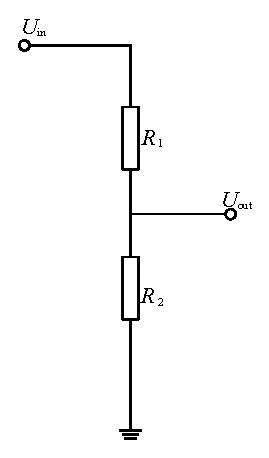
\includegraphics{grafiken/2.1.eps}
	\caption{Structure of divider resistor} 
	\label{fig:2.1}
\end{figure}
Here, $\cdot U_{in}$ is the voltage of component under test, $\cdot U_{out}$ is voltage of divider resistor R2, and $\cdot R_{1}$, $\cdot R_{2}$ are divider resistors.
\\
Therefore, the measured voltage provided to the ADC channel is the following formula:
\\
\begin{center} 
\begin{equation}
 U_{out} = \frac{R_{2}}{R_{1}+R_{2}} U_{in}  
\end{equation}
\end{center}

There are a variety of precision ADCs available on the market to choose from, as shown in the Figure~\ref{fig:2.2} below , the appropriate ADC precision can be selected according to the signal bandwidth, so that it is convenient for users to measure.
\begin{figure}[h]
	\centering
	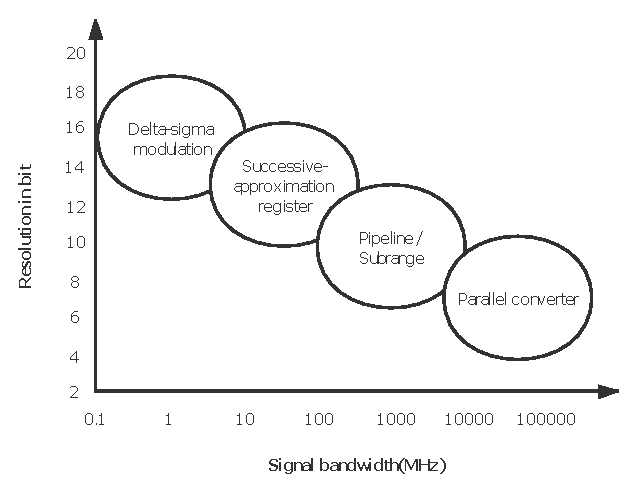
\includegraphics{grafiken/2.2.eps}
	\caption{ADC-Architecture depending on signal bandwidth and resolution} 
	\label{fig:2.2}
\end{figure}
\\
In the case of methods without feedback, the parallel converter has the simplest structure, which is why, with high resolution, a large number of components with high demands on accuracy are required. Here, too, there are methods with range selectivity, oversampling and ramp methods. A folding process has also established itself alongside a multiplex technique. 
\\
The following Figure~\ref{fig:2.3} briefly describes the basic structure of the parallel converter:
\begin{figure}[h]
	\centering
	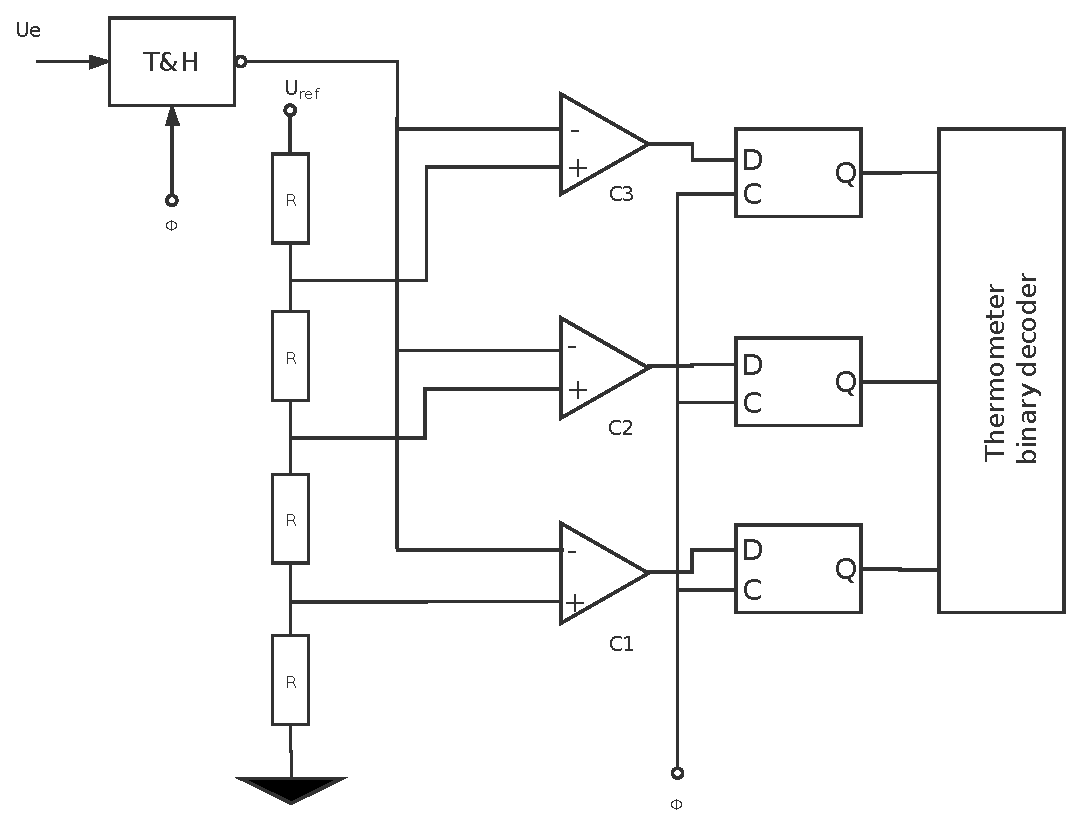
\includegraphics[width=15cm]{grafiken/2.3.eps}
	\caption{Block diagram of a parallel converter} 
	\label{fig:2.3}
\end{figure}
\\
Since with this parallel converter (flash converter) the entire conversion takes place within one clock period, it is the fastest method. It is easy to see, however, that the number of components required quickly becomes very large, since the entire chain with resistor, comparator and latch is required for each of the $2^{n}-1$ comparison values. The thermometer code present at the output of the latches is encoded in a binary code (often a Gray code, in which neighboring numbers differ by only one bit). Differential amplifiers are particularly suitable as comparators, with the gain v having to be at least so large that $\Delta U/2$ is sufficient to control the necessary logic level of the latches.
\\
The second important method is called the weighing method, which requires feedback via a digital-to-analog converter, as Figure ~\ref{fig:2.4} shows.
\begin{figure}[h]
	\centering
	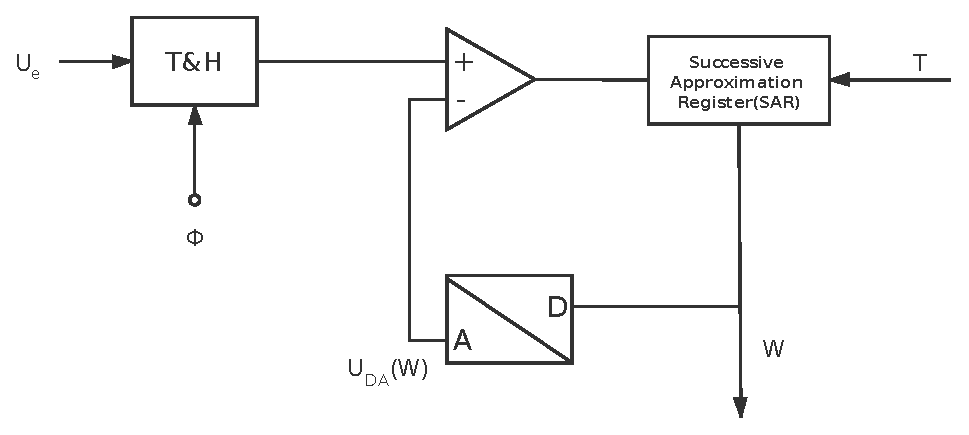
\includegraphics{grafiken/2.4.eps}
	\caption{Converter according to the weighing method} 
	\label{fig:2.4}
\end{figure}
 As soon as the track and hold element (T\&H) has switched to hold mode, the weighing cycle begins with the most significant bit. If $ u_{e}>\frac{U_{max}}{2} $, the top bit remains set and the second bit is set to 1 on a trial basis.
\\
The comparator decides whether the word in the SAR is smaller than the input signal. Then the check bit remains set and the next lowest bit is checked. If  $u_{e}<u_{DA}(W)$, the check bit is reset.
\\
The conversion time is n clock periods, whereby the digital-to-analog converter must have full accuracy. The advantage of high resolutions is that only one precise comparator is required. This enables the design of very energy efficient implementations.
If a counter is used instead of the SAR, the Laund can count the clock cycles backwards through the comparator. In the steady state, the data word indicates. There are also many variants of this counting method, whereby in the worst case the conversion time can be up to $2^{n}$ clock cycles.
In the gallium nitride measurement, because the precision is required but the precision is not the highest, the above-mentioned method is selected.

\subsection{ADC in microcontroller STM32F303ZET}
\label{sec:ADC in microcontroller STM32F303ZET}
% 2.1.2
In this measurement, we choose STM32F303ZET as a microcontroller containing multiple 12-bit precision ADCs. Its core is ARM-Cortex-M4, and its ADC is of type Successive approximation register.
Each stm32F303 has a 40-channel independent 16-bit precision ADC, and the price is very high, so we choose this microcontroller to measure the voltage signal to determine whether the gallium nitride is affected by cosmic rays. The following Figure~\ref{fig:2.5} is the typical connection diagram using the ADC:
\begin{figure}[h]
	\centering
	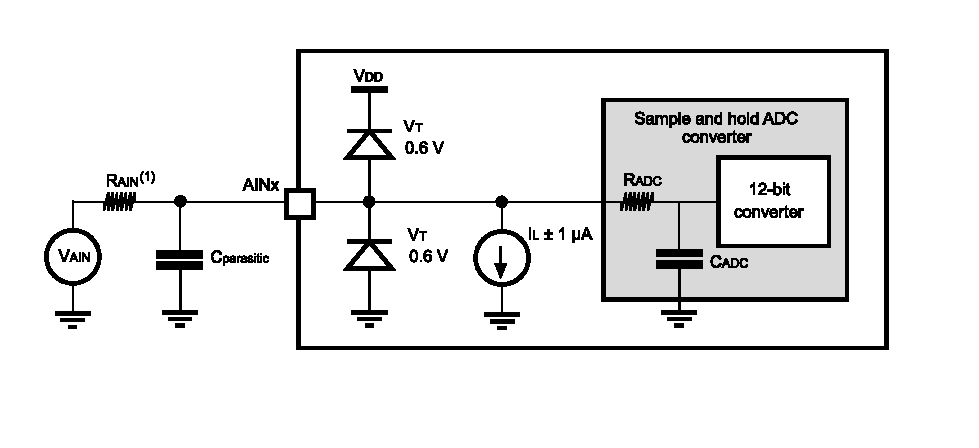
\includegraphics{grafiken/2.5.eps}
	% datasheet 144/173
	\caption{Typical connection diagram using the ADC} 
	\label{fig:2.5}
\end{figure}
\section{Ethernet}
\label{sec:Ethernet}
% 2.2
Ethernet has very extensive and in-depth applications in various fields and industries. This is mainly due to the high flexibility and ease of implementation of Ethernet. Because Ethernet has the advantages of simple networking, low cost, excellent compatibility, reliable connection, and convenient topology adjustment, it has advantages that other network technologies do not have in terms of being a gateway for smart homes, Internet of Things or wireless sensor networks. , Thus get vigorous development and application. This article will introduce in detail how to connect the embedded system to the Ethernet, how to use the hardware protocol stack to make your solution or application connect to the Internet quickly and efficiently, how to realize TCP/IP communication, and how to realize the upper application layer protocol and many more.
\subsection{Introduce of W5500}
\label{sec:Introduce of W5500}
% 2.2.1
The W5500 network expansion board integrates a hardware TCP/IP protocol stack chip W5500 and an RJ-45 with a network transformer. Among them, W5500 is a full hardware TCP/IP embedded Ethernet controller, which provides a simpler Internet connection solution for embedded systems. Hardware logic gate circuits are used to implement the transmission layer and network layer of the TCP/IP protocol stack (such as : TCP, UDP, ICMP, IPv4, ARP, IGMP, PPPoE and other protocols), and integrates the data link layer, physical layer, and 32K bytes of on-chip RAM as a data receiving and sending buffer. Make the host computer main control chip only need to undertake the processing task of TCP/IP application layer control information. This greatly saves the workload of the host computer for data replication, protocol processing, and interrupt processing, and improves system utilization and reliability. 
\\
Its module structure is shown in the Figure~\ref{fig:2.6} below:
\\
\begin{figure}[h]
	\centering
	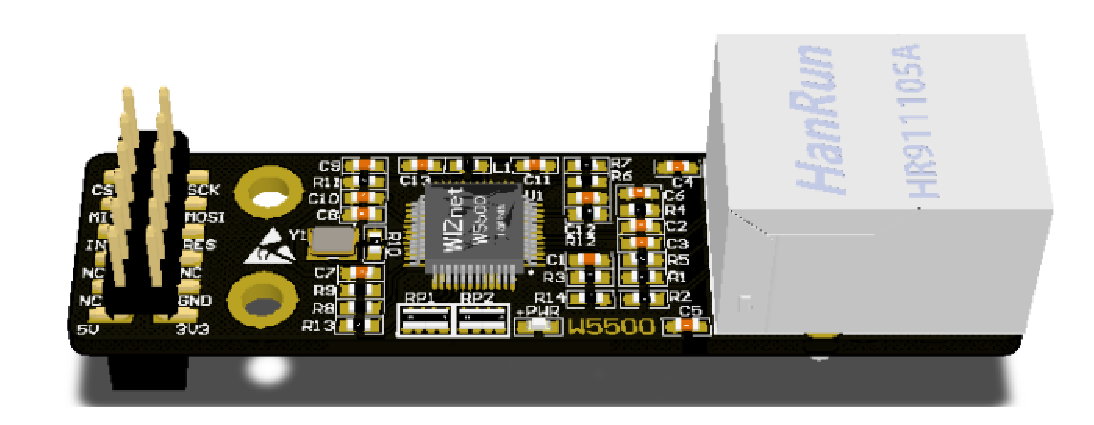
\includegraphics[width=15cm] {grafiken/2.6.eps}
	\caption{Physical model of W5500} 
	\label{fig:2.6}
\end{figure}
W5500 supports 8 sockets at the same time to facilitate communication with different IPs and devices; in order to reduce system energy. W5500 provides Wake-on-LAN mode (WOL) and power-down mode for customers to choose to use; W5500 is non-aggressive. The hardware network engine can prevent similar torrent, fraud and injection network attacks and improve network security.

\subsection{solution of ethernet access}
\label{sec:solution of ethernet access}
% 2.2.2
For non-operating system, how does the single-chip microcomputer required by the system realize network access? I will categorize these schemes according to the different TCP/IP protocol stacks below.
\\
It is divided into two categories: the first category is the traditional software TCP/IP protocol stack solution; the second category is the latest hardware TCP/IP
Protocol stack scheme. Below I will analyze the implementation of these two types of solutions: 
\\
1) MAC+PHY solutions:

\begin{figure}[!ht]
	\centering
	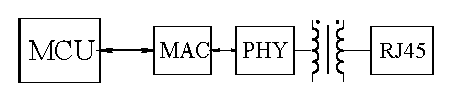
\includegraphics[width=15cm] {grafiken/2.7.eps}
	\caption{MAC+PHY Ethernet solution} 
	\label{fig:2.7}
\end{figure}
\FloatBarrier
The traditional Ethernet access scheme is as shown in the figure below. The MCU+MAC+PHY is added to the network interface to realize the Ethernet
The physical connection of the network realizes communication and upper-layer applications by implanting TCP/IP protocol code in the main control chip.
\\
2) Hardware protocol stack chip solution: 
\begin{figure}[!ht]
	\centering
	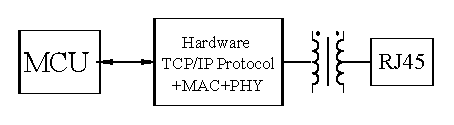
\includegraphics[width=15cm]{grafiken/2.8.eps}
	\caption{Hardware protocol stack chip solution} 
	\label{fig:2.8}
\end{figure}
\FloatBarrier
The hardware protocol stack chip scheme is shown in the figure below. The MCU + hardware protocol stack chip (including MAC and PHY) directly adds the network interface, and the single-chip microcomputer can be easily connected to the network. All the work of processing the TCP/IP protocol is through the "little secretary" of the MCU-the hardware protocol Stack chips to complete.
\\
This solution was first proposed by WIZnet and successfully launched the Ethernet series of chips: W5100, W5200, W5300 and W5500. The so-called hardware protocol stack refers to the implementation of the traditional software TCP/IP protocol stack with hardware-based logic gate circuits, as shown in the Figure~\ref{fig:2.9} below.
\begin{figure}[!ht]
	\centering
	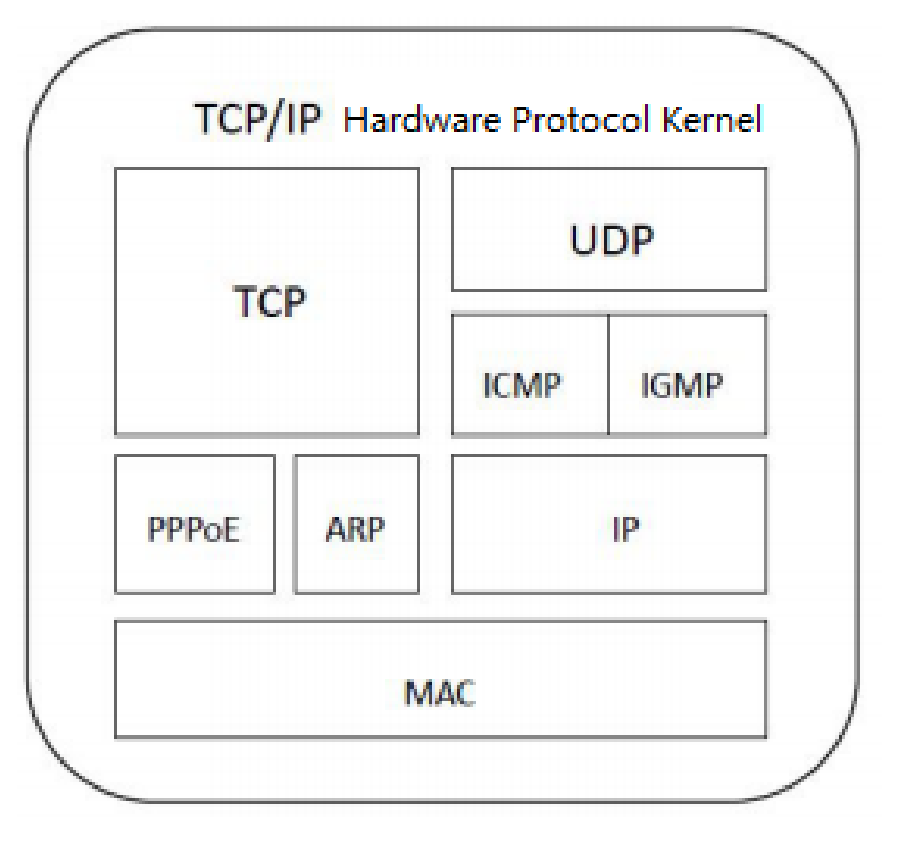
\includegraphics[scale=0.85]{grafiken/2.9.eps}
	\caption{Hardware protocol kernel} 
	\label{fig:2.9}
\end{figure}
\FloatBarrier
The core of the Ethernet chip is composed of protocols such as TCP, UDP, ICMP, IGMP in the transport layer, IP, ARP, PPPoE and other protocols in the network layer, and MAC in the link layer, plus physical layer PHY and peripheral registers and memory The SPI interface constitutes this complete set of hardware-based Ethernet solutions.
\\
This hardware TCP/IP protocol stack replaces the previous MCU to handle these interrupt requests. That is, the MCU only needs to process user-oriented application layer data. The transmission layer, network layer, link layer and physical layer are all controlled by the peripheral WIZnet The chip is complete. This set of solutions simplifies the aforementioned five-layer network model from two aspects of hardware overhead and software development, and simplifies product development solutions. In this way, engineers no longer have to face the cumbersome communication protocol code, only need to understand the simple register function and Socket programming to complete the network function development part of the product development work.

\section{SMTP}
\label{sec:SMTP}
% 2.10
When collecting temperature signals, if the state of more than 50 units under test suddenly changes within 10s, it is likely to be a manual error. At this time, it is necessary to set up an email-related program in the measurement system to send an email to notify the researcher. This article uses the SMTP protocol.
SMTP stands for Simple Mail Transfer Protocol. It is a group of mails used to transfer mail from source address to destination address
Rules, which control the way in which letters are transferred. The actual process of sending emails can be shown in Figure~\ref{fig:2.10}:
 
% ~\ref{fig:2.10} 
\begin{figure}[!ht]
	\centering
	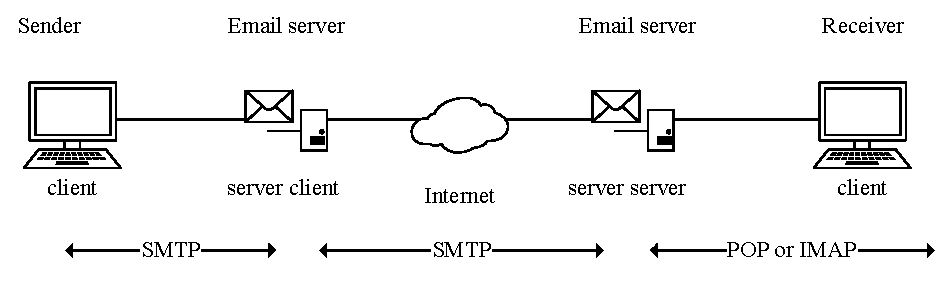
\includegraphics[width=15cm]{grafiken/2.10.eps}
	\caption{Schematic diagram of the mail sending process} 
	\label{fig:2.10}
\end{figure}
\FloatBarrier

An important feature of it is that it can relay mail during transmission, that is, mail can be relayed through hosts on different networks. Usually it works in two situations: one is the transmission of mail from the client to the server; the other is the transmission from one server to another server. SMTP is a request/response protocol, it monitors port 25, is used to receive the user's Mail request, and establish an SMTP connection with the remote Mail server.
\\
SMTP usually has two working modes. Send SMTP and receive SMTP. The specific working method is: Send SMTP after receiving the user's mail request, determine whether the mail is a local mail, if it is directly delivered to the user's mailbox, otherwise query the MX record of the remote mail server to the DNS, and establish a connection with the remote A two-way transmission channel between receiving SMTP, after which SMTP commands are issued by the sending SMTP, received by the receiving SMTP, and the response is transmitted in the opposite direction. Once the transmission channel is established, the SMTP sender sends a MAIL command to indicate the sender of the mail. If the SMTP receiver can receive the mail, an OK response is returned. The SMTP sender then issues the RCPT command to confirm whether the mail has been received. If the SMTP receiver receives it, it will return an OK response; if it cannot receive it, it will send a rejection response (but not stop the entire mail operation), and both parties will repeat this many times. When the receiver receives all the mails, it will receive a special sequence. If the receiver successfully processes the mail, it will return an OK response.
\\


\section{UDP}
\label{sec:UDP}
% 2.4
In the transport layer of the TCP/IP protocol stack, TCP is connection-oriented, and the UDP protocol to be demonstrated next. It is non-connection oriented.
\\
When UDP transmitting data, there is no confirmation, retransmission, or congestion mechanism. Since this measurement can obtain a large amount of data in a short time, the packet loss and error data can be verified by the large amount of data received later, so this time we choose UDP.
\\
Compared with TCP, UDP does not return a response signal for each received frame during transmission. When network transmission fails, such as a router restart and the network is suddenly interrupted, UDP can still receive the signal transmitted by the server as much as possible. The comparison figure~\ref{fig:2.11}  is as follows :
% ~\ref{fig:2.11} 
\begin{figure}[!ht]
	\centering
	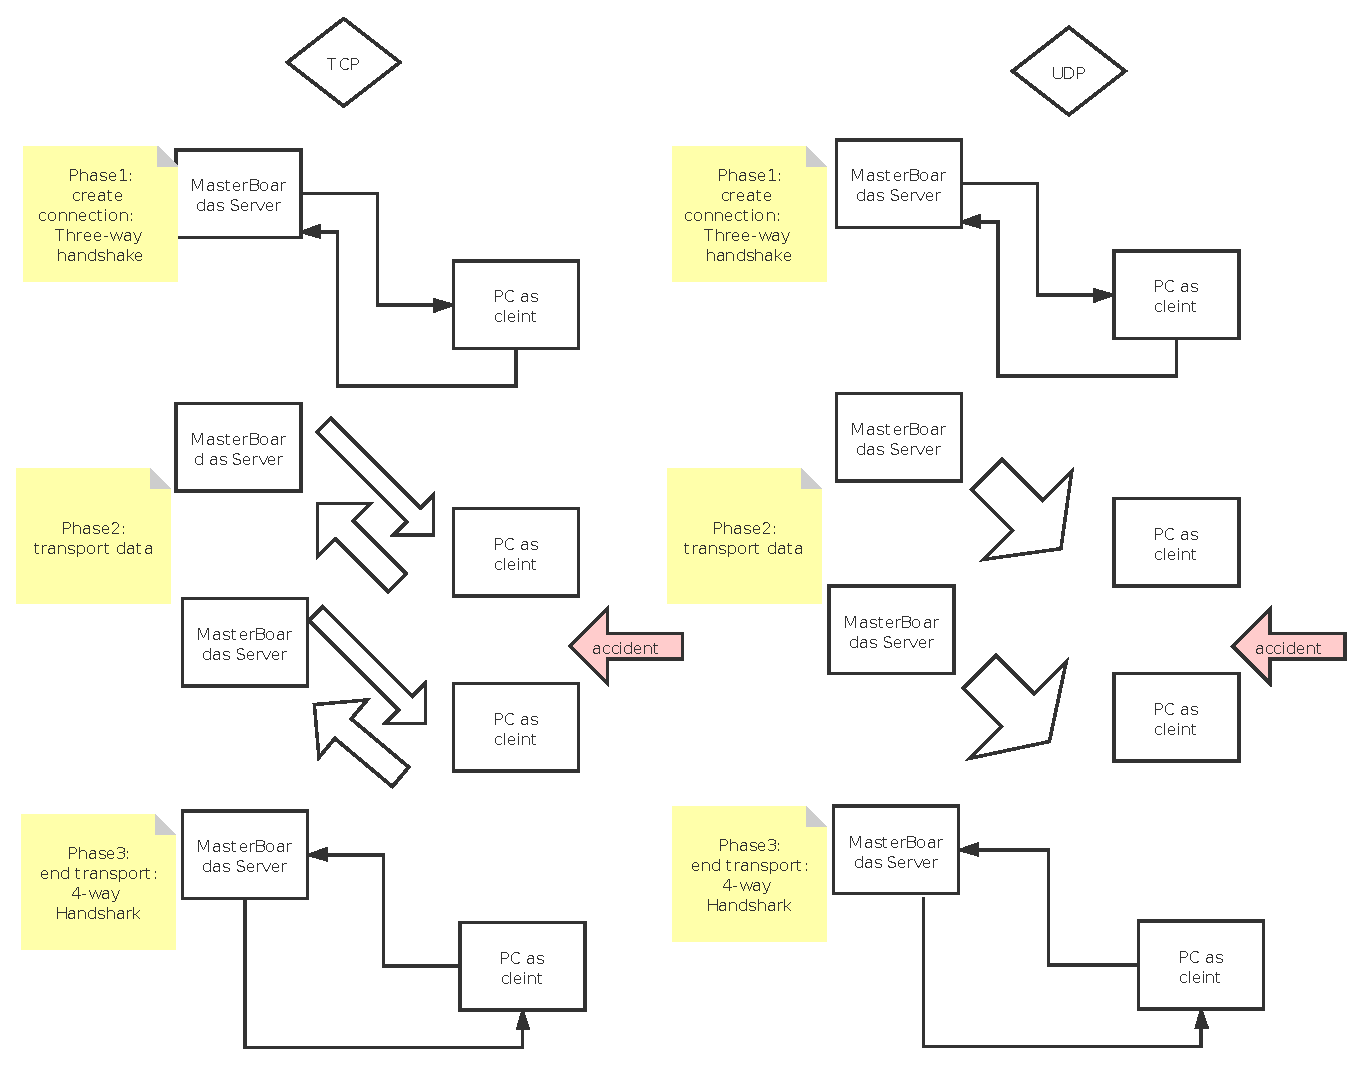
\includegraphics[scale=0.7]{grafiken/2.11.eps}
	\caption{Comparison of TCP and UDP} 
	\label{fig:2.11}
\end{figure}
\FloatBarrier
The UDP establishment process of W5500 is also very convenient, which can be easily realized by simply reading and writing registers. After the program is initialized, enter the main loop function. When the Socket is closed, before communicating, we first initialize the Socket port in UDP mode. When the socket is in the initialization completed state, that is, the SOCK UDP state, data can be sent by broadcast at this time.
\\
Next, use W5500 to demonstrate how to use UDP to send and receive data. There are two issues to pay attention to before the test. 
\\
First, it is recommended to turn off the PC firewall.
\\
Secondly, if the W5500 module and the PC are directly connected via a network cable, you need to modify the IP address of the PC to a static IP, and keep it in the same network segment as the W5500 IP. 
\\
If you connect to the router directly, you do not need to modify the IP address of the PC. The specific test steps are:
\\
1. Use the IP address obtained by the router to set the configuration file in the W5500, this IP must be in the same network segment as the router gateway.
\\
2. Obtain the computer IP address through the command line and write it as remote IP into the configuration file of the w5500 Ethernet chip.
\\
3. Compile the code, and then burn the program to the Wildfire development board.
\\
4. Connect the network cable and USB serial port cable. Open the serial port debugging tool, reset the Wildfire development board, and get the setting information from the output result.

\section{SPI}
\label{sec:SPI}
% 2.5
The Serial Peripheral Interface (SPI) is a synchronous serial communication interface specification used for short-distance communication, primarily in embedded systems. The interface was developed by Motorola in the mid-1980s and has become a de facto standard. Typical applications include Secure Digital cards and liquid crystal displays.
\\
SPI devices communicate in full duplex mode using a master-slave architecture with a single master. The master device originates the frame for reading and writing. Multiple slave-devices are supported through selection with individual slave select (SS), sometimes called chip select (CS), lines.
\\
Sometimes SPI is called a four-wire serial bus, contrasting with three-, two-, and one-wire serial buses. The SPI may be accurately described as a synchronous serial interface,[1] but it is different from the Synchronous Serial Interface (SSI) protocol, which is also a four-wire synchronous serial communication protocol. The SSI protocol employs differential signaling and provides only a single simplex communication channel. SPI is one master and multi slave communication.
\\
The figure~\ref{fig:2.12}  below is a standard SPI transmission process:
% ~\ref{fig:2.11} 
\begin{figure}[!ht]
	\centering
	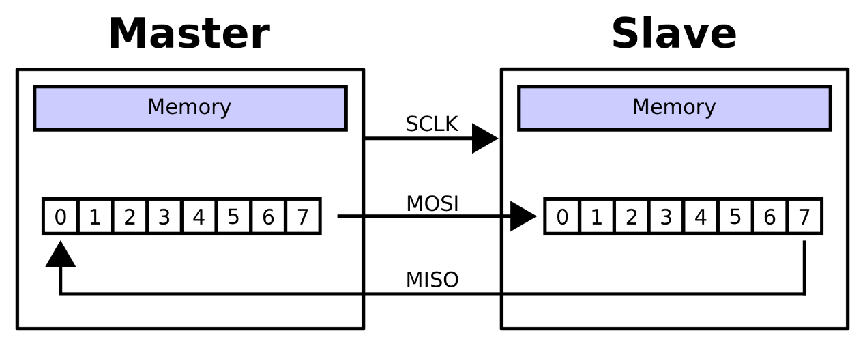
\includegraphics[width=15cm]{grafiken/2.12.pdf}
	\caption{standard SPI transmission process} 
	\label{fig:2.12}
\end{figure}
\FloatBarrier

\section{DMA}
\label{sec:DMA}
% 2.6
The basic definition of DMA: 
DMA has the full name of Direct Memory Access 
DMA transmission copies data from one address space to another address space, so as to realize high-speed data transmission between peripherals and memories or between memories. When CPU initializes such a transmission action, the transmission action is realized and completed through the DMA controller. The DMA transmission mode is dispense with CPU to realize direct control transmission or differing from the interrupt processing mode, it will reserve the site and recover the site process. Through RAM and IO devices, a channel of direct transmission data can be opened to improve CPU efficiency strongly. 

Main features of DMA:
Each channel is directly connected with the exclusive hardware DMA request. Each channel also supports software touch. Such functions can be configured through software; 
On the same DMA module, the priority between multiple requests can be established through software programming (with a total of four levels: very high, high, medium, and low). When the priority setting is equal, it depends on hardware (request 0 precedes over request 1, and the rest may be deduced by analogy); 
For the transmission width of independent data sources and target data areas (byte, half-word, and full-word), byte control is used in this design to simulate the process of packing and unpacking. The source and target address must be aligned according to the data transmission width; 
The buffer management can support circulation; 
Each channel has three event flags (DMA semi-transmission, DMA transmission completion, and DMA transmission error). The logic of three event flags may become an individual interrupt request; 
Transmission between memories, transmission between peripherals and memories, and transmission between memories and peripherals; 
Flash memory, SRAM, SRAM of peripherals, APB1, APB2, and AHB peripherals can be used as sources and targets for access; 
The maximum number of programmable data transmission is 65535. 
STM32F429 series chip DMA controller 
STM32F429 series chip at most has two DMA controller. DMA1 and DMA2 respectively includes 8 channels. Each channel specializes in managing the request of one or multiple peripheral for memory access. It also has the priority of coordinating each DMA request through arbitration. 

For the requests generated from peripherals (TIM, ADC, SPI1, SPI/I2S2, I2C and USART), it is inputted to DMA1/DMA2 controller through logic, implying that only one request is valid at the same time. 
DMA’s work block diagram is stated below: 
~\ref{fig:2.13}  of DMA:
% ~\ref{fig:2.12} 
\begin{figure}[!ht]
	\centering
	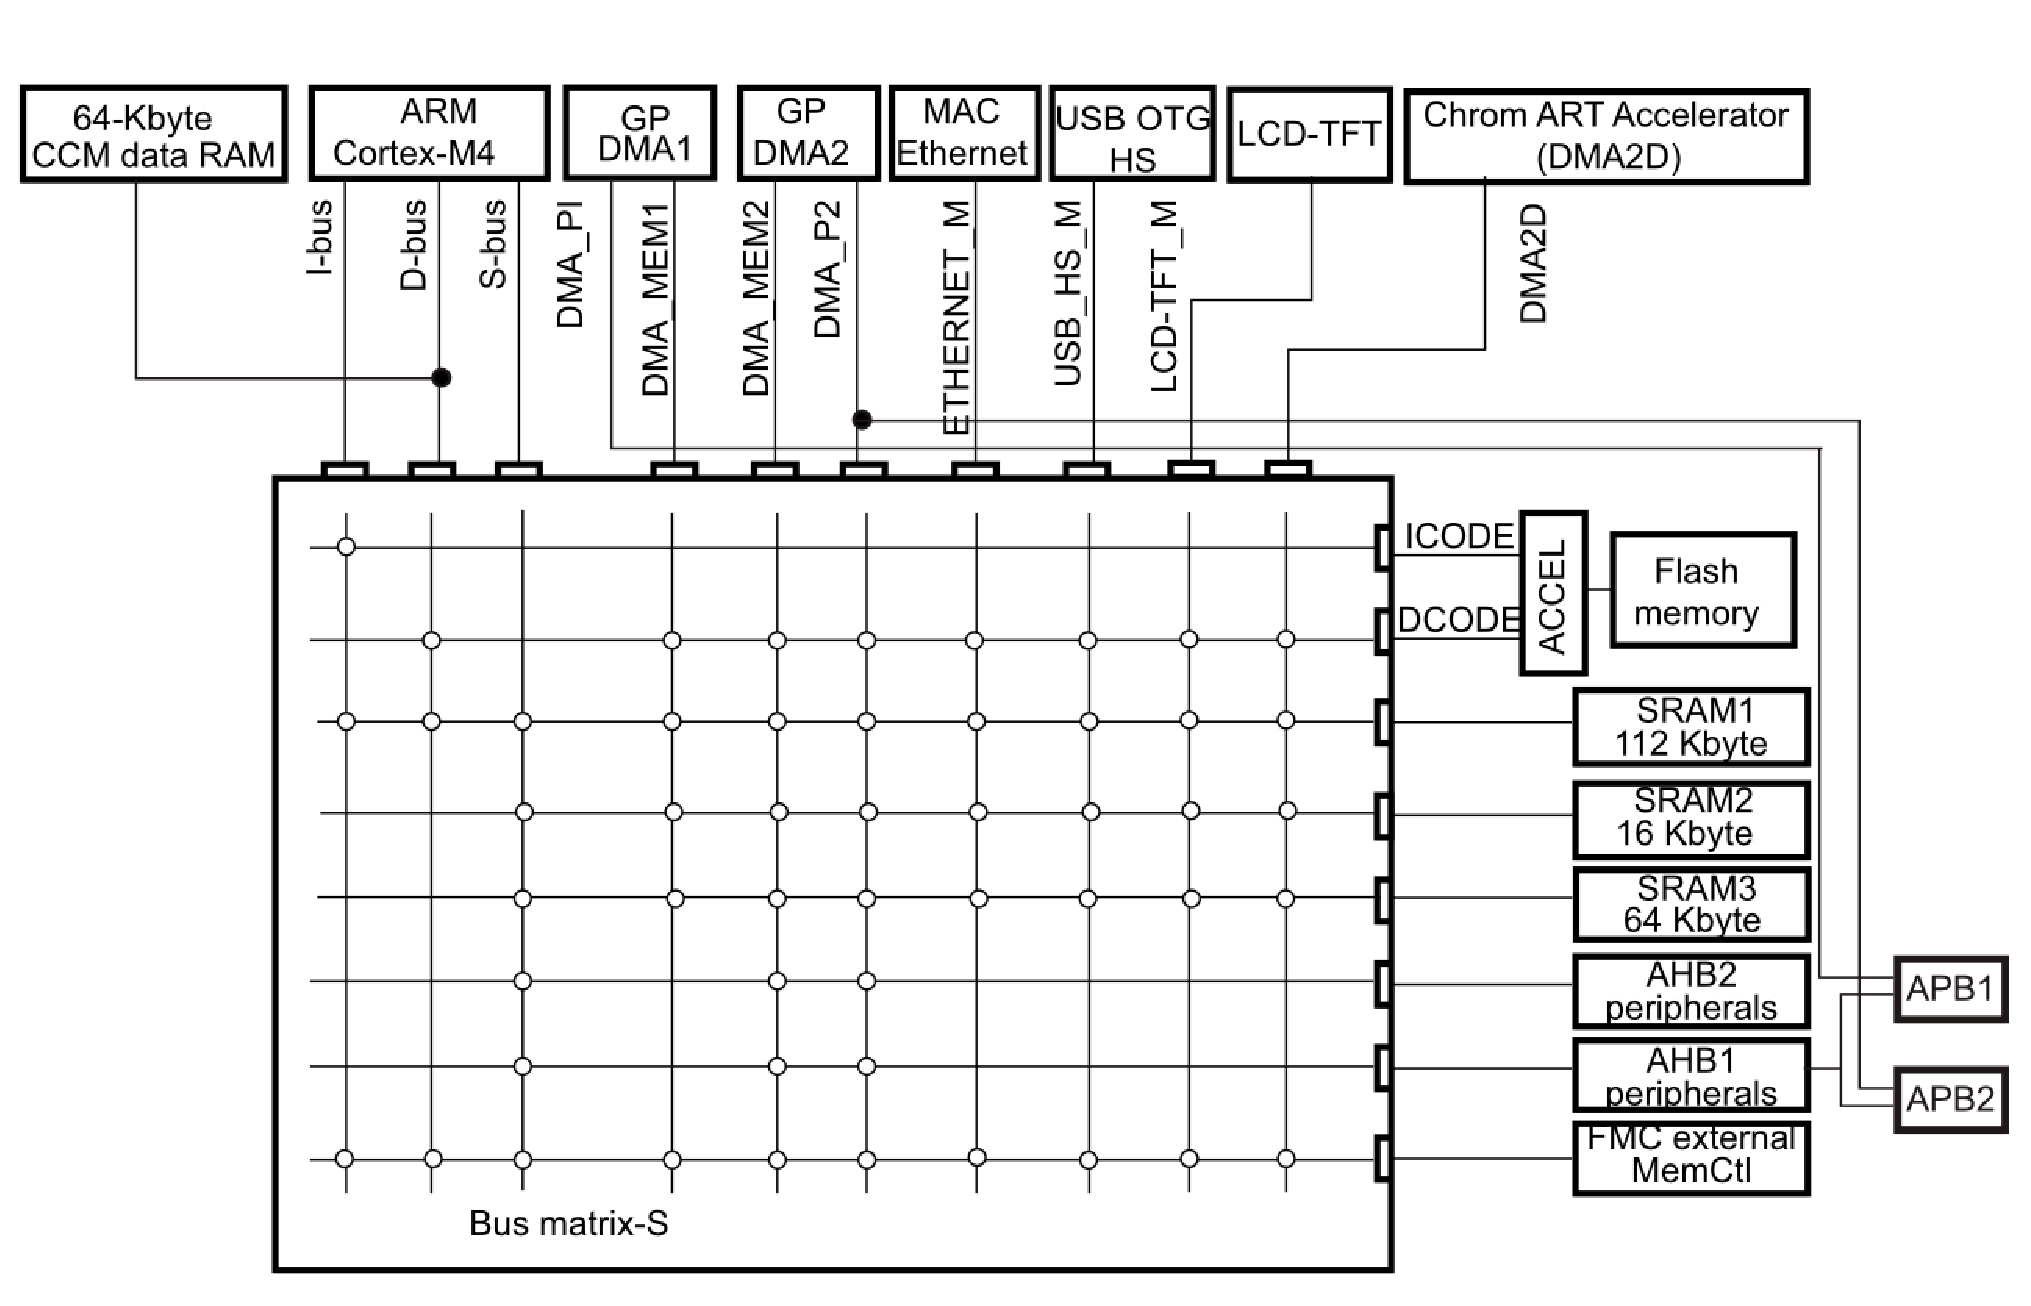
\includegraphics[width=15cm]{grafiken/2.13.eps}
	\caption{STM32F429xx Multi-AHB matrix} 
	\label{fig:2.13}
\end{figure}
\FloatBarrier

\section{Ngrok}
\label{sec:Ngrok}
% 2.7
Internal network penetration or NAT penetration aims to make the data package with a specific source IP address and source port number not block from NAT but will route to the internal network host correctly. The internal network penetration method is introduced through the relative position between the mutual communication host in the network and NAT devices. 
The UDP’s internal network penetration, in essence, uses the NAT system on the router. NAT is a conversion technology that transforms the private (reserved) address into the legal IP address. It is widely applied in the internet access ways with all kinds of types and different types of networks. NAT can reuse the address and realize external shelter for the internal network structure. 
Ngrok is a commonly used internal network penetration technology. Generally speaking, our local PC has two IPv4 addresses. One local IP is allocated by the router and the other one is the public network IP. However, people in other areas all over the world cannot directly use such two IP addresses to access the local PC. If the project’s logic and data structure are not complicated, developers can use the open-source ngrok for the internal network penetration so that external personnel can access the local PC. 
The following Figure~\ref{fig:2.14}  is a common application structure diagram of NAT.
% ~\ref{fig:2.14} 
\begin{figure}[!ht]
	\centering
	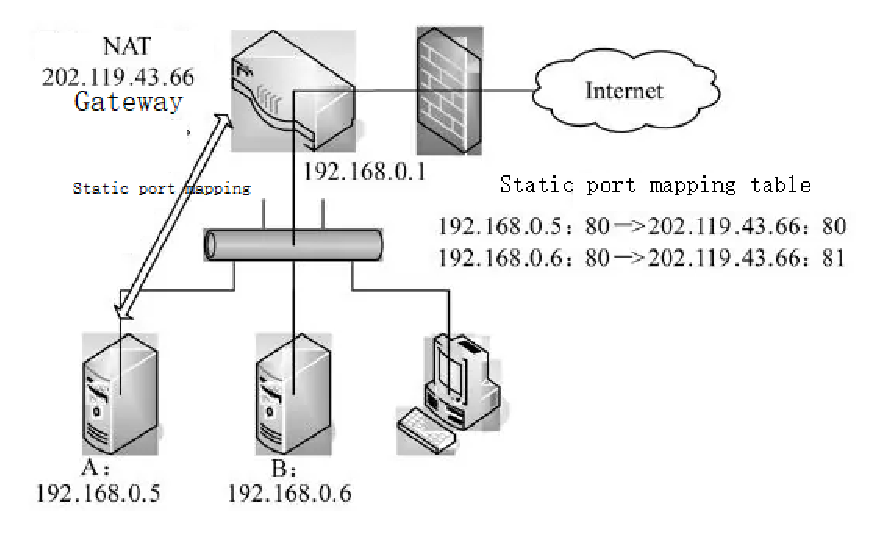
\includegraphics {grafiken/2.14.eps}
	\caption{NAT-Technical} 
	\label{fig:2.14}
\end{figure}
\FloatBarrier
This article uses Ngrok for intranet penetration, the structure is as follows Figure~\ref{fig:2.15} :

% ~\ref{fig:2.15} 
\begin{figure}[!ht]
	\centering
	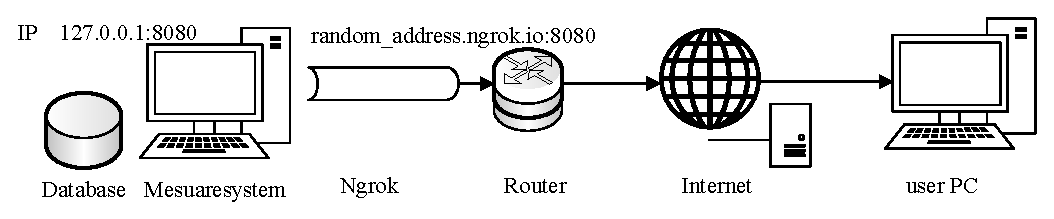
\includegraphics[width=15cm]{grafiken/2.15.eps}
	\caption{Ngrok-Technical realization} 
	\label{fig:2.15}
\end{figure}
\FloatBarrier

\section{IoT}
\label{sec:IoT}
% 2.8
Internet of Things is abbreviated into IoT. 
In brief, it means that all devices are linked to the internet in a way: 
From smartphones and tablet PCs (common) to automobiles and refrigerators 
The main function of IoT lies in how to link devices, services, and Apps to the internet so that it will develop the greater role. There is almost no limitation for devices accessed in the internet and reasons for access. 
The important way for IoT to improve quality of life lies in making data sharing easier. IoT is conducive to streamlining our life. In the long term, it can handle some trifling matters for us. 
This article uses the core philosophy of IoT and issues data collected to the cloud. Users can access the cloud server through HTML5 page to gain the pushed data. If the cloud server breaks down, user PC can collect the PC through VNC remote control. 

The signal collector gains the outer net IP as the server through internal network penetration. The signal collected by the single chip microcomputer through UDP is imported to the database. Users or researchers in other areas can gain the database data of the signal collector through the html webpage (deployed on the free website of githubpage). When the signal collector goes wrong, users can collect the signal machine through VNC remote control. 

The following Figure~\ref{fig:2.16} is a schematic diagram of the Internet of Things structure used in this article:
% ~\ref{fig:2.16} 
\begin{figure}[!ht]
	\centering
	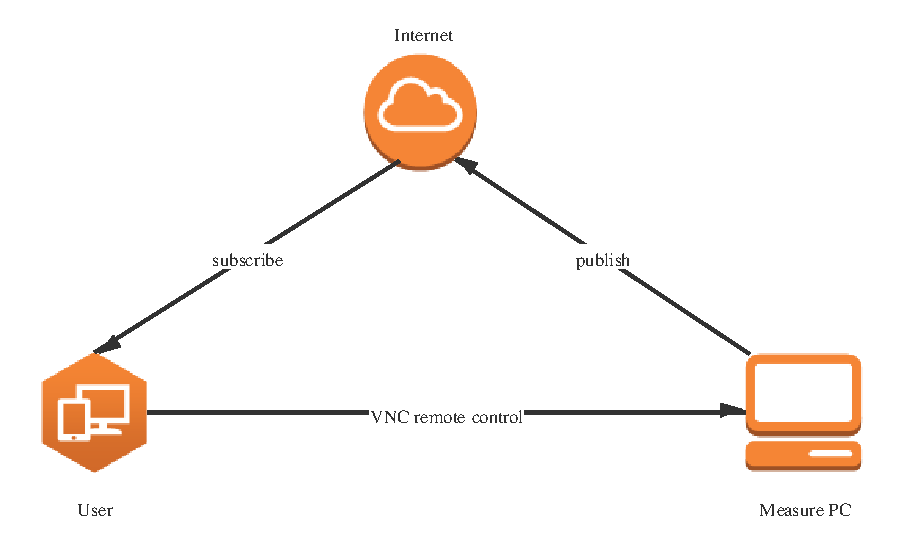
\includegraphics[width=15cm]{grafiken/2.16.pdf}
	\caption{Measuring models using the Internet of Things} 
	\label{fig:2.16}
\end{figure}
\FloatBarrier

The signal acquisition machine obtains the external network IP as a server through the intranet penetration, and collects the signal collected by the single-chip microcomputer through UDP and imports it into the database. Users or researchers in other regions can obtain it through the html web page (which has been deployed on the free website of the github page) Collect the database data of the signal machine. When there is a problem with the signal machine, the user can also remotely control the signal machine through VNC.

 
\chapter{Introduction of measurement circuit}
\label{chap:Introduction of measurement circuit}
% 3.0
This article mainly studies the influence of voltage, current, and temperature on gallium nitride to determine the influence of cosmic rays on gallium nitride. At the same time, the voltage signal and current signal of the measured unit are equivalent. Because of Ohm's law, voltage and current are proportional, so in this measurement process, this article mainly measures the change of voltage and temperature. When cosmic rays affect gallium nitride, the source and drain of gallium nitride are turned on and enter triode mode or saturation mode, that is, gallium nitride cannot work normally because of cosmic rays.

In order to ensure the measurement accuracy, we add an ADC in front of the unit under test. If the gallium nitride is affected by cosmic rays, the ADC measurement value will change from high to low to achieve the measurement purpose. 
\\
\section{Measurement circuit overview}
\label{sec:Measurement circuit overview}
% 3.1
\\
% The following figure shows the basic structure of the measurement system, which is blown using a fuse.
For multiple units under test, we adopt a one-to-one correspondence method, that is, each unit under test corresponds to an ADC for voltage measurement, and IGBT is used as a protection circuit.
The Figure~\ref{fig:3.1} below shows the basic structure of a measurement system for multiple DUTs.
\\
\begin{figure}[!ht]
	\centering
	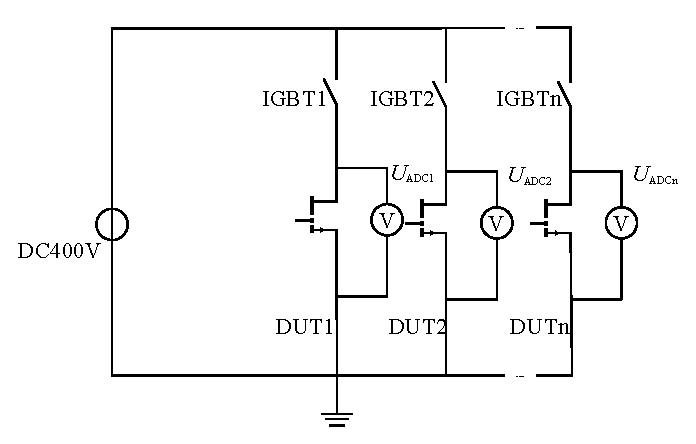
\includegraphics[width=15cm]{grafiken/3.1.eps}
	\caption{Basic structure of the measurement system for multiple DUTs} 
	\label{fig:3.1}
\end{figure}
\FloatBarrier
\\
% When DUT is disturbed by the cosmic rays and it is conductive, the basic circuit uses the fuse as the action circuit. Then, the measuring signal chip suddenly gains a high level and remains the high level. Next, the software system adds one for the error signal counter. The basic constitution of the measuring circuit is shown in Figure  : 
% \\
% In actual use, if we do not consider IGBT control, we can use IGBT as the protecting circuit component. When fusing of the gallium nitride MOSFET is affected by cosmic rays and it is conductive, the microcontroller can gain the voltage value through ADC, so as to realize whether the gallium nitride component will be influenced. The artificial circuit is illustrated below: 
% When DUT is normally operated, IGBT in theory gains a 0V voltage and it will not turn on the microcontroller to get a low level, as shown below: 
% \\
% When DUT is unusually operated, IGBT in theory gets a 15V voltage(with IGBT breakover) and it will not turn on the microcontroller to get a high level, as shown below: 
\\
\section{IC for IGBT control circuit}
\label{sec:IC for IGBT control circuit}
% 3.2
LM393 voltage comparator is used to control IGBT 
LM393 is a common voltage comparator chip in our daily life. It has two independent operational amplifiers. The power supply is provided by wide voltage and undercurrent. Low input controls the current. Generally speaking, the actuation time only has 1.3 microseconds. When the in-phase input voltage is greater than the inverted input voltage, output voltage belongs to the high level. When the in-phase input voltage is less than the inverted input voltage, output voltage belongs to the low level. 

The following Figure~\ref{fig:3.2} is a common application circuit of LM393.

\begin{figure}[!ht]
	\centering
	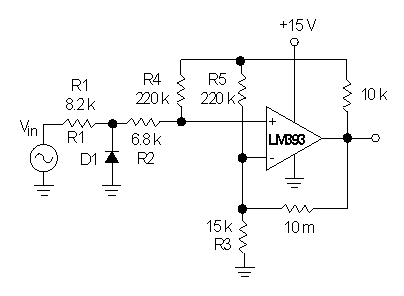
\includegraphics[width=13cm]{grafiken/3.2.eps}
	\caption{Application circuit of LM393} 
	\label{fig:3.2}
\end{figure}
\FloatBarrier
\\
\section{Simulation circuit}
\label{sec:Simulation circuit}

% 3.3
In order to design the measurement system correctly, this article uses matlab's simlink to simulate and analyze the results.
The basic constitution of the measuring circuit is shown in Figure~\ref{fig:3.3}:
\begin{figure}[!ht]
	\centering
	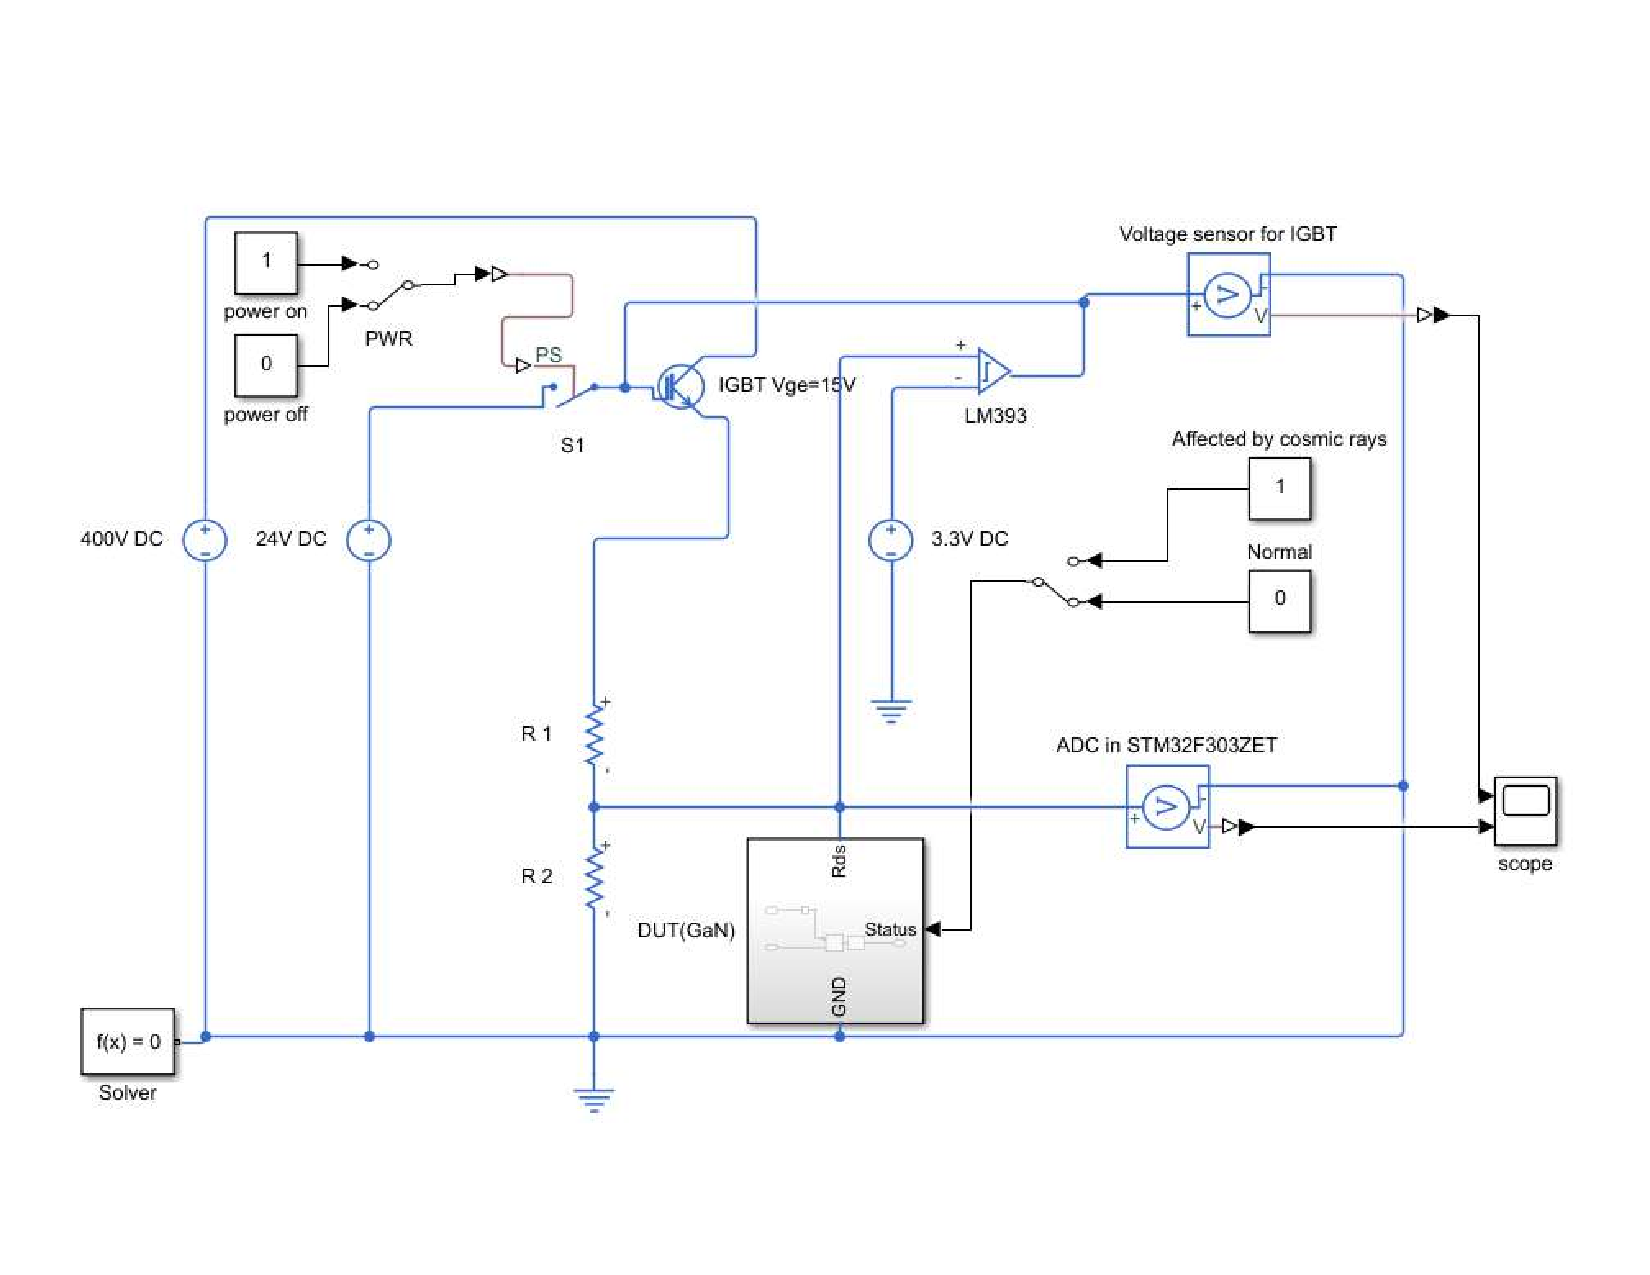
\includegraphics[width=17cm]{grafiken/3.3.pdf}
	\caption{basic constitution of the measuring circuit} 
	\label{fig:3.3}
\end{figure}
\FloatBarrier
\\
Among them, $R_{1}$ and $R_{2}$ are voltage divider circuits to ensure that the voltage across $R_{2}$ exceeds 3.3V under normal conditions. At this time, the voltage across R2 is greater than Non-inverting input of LM393(3.3V), which can ensure that the output of the LM393 output is greater than or equal to a high level of 15V, forming a self-locking circuit. For long-term measurement, it is not necessary to apply external voltage to pushbutton S1.
\\
In order to turn on the igbt for measurement, the pushbutton S1 need to be press 
at the beginning, since the circuit is self-locking, the gate voltage of the IGBT is always 15V, if the status of DUTs are normal. The measurement
status changes are shown in the following Table~\ref{tab:3.1}:
 
\begin{table}[]
\begin{tabular}{@{}|l|l|l|l|l|l|l|@{}}
\toprule
\rowcolor[HTML]{EFEFEF} 
Status                      & V+ & V-(as Vref) & Vout & IGBT     & ADC  & ADC Value \\ \midrule
DUT normal                  & 0V & >3.3V       & 15V  & turn on  & 0V   & 0         \\ \midrule
DUT affected by cosmic rays & 0V & 3.3V        & 0V   & turn off & 3.3V & 4095      \\ \bottomrule
\end{tabular}
	\caption{Measuring system status and voltage changes}
	\label{tab:3.1}
\end{table}

 
\\
When the DUT is affected by cosmic rays, because the internal resistance of the GaN-MOSFET is very small(less than $63m\Omega$), the voltage across $R_{2}$ drops rapidly and approaches 0. At this time, the Non-inverting input of LM393 is less than 3.3V at the inverting input, and the comparator The output voltage is 0. At this time, the gate voltage of the IGBT is 0, and the IGBT cannot be turned on. In this way, the IGBT protection circuit can normally protect the malfunctioning DUT.




\begin{figure}[!ht]
	\centering
	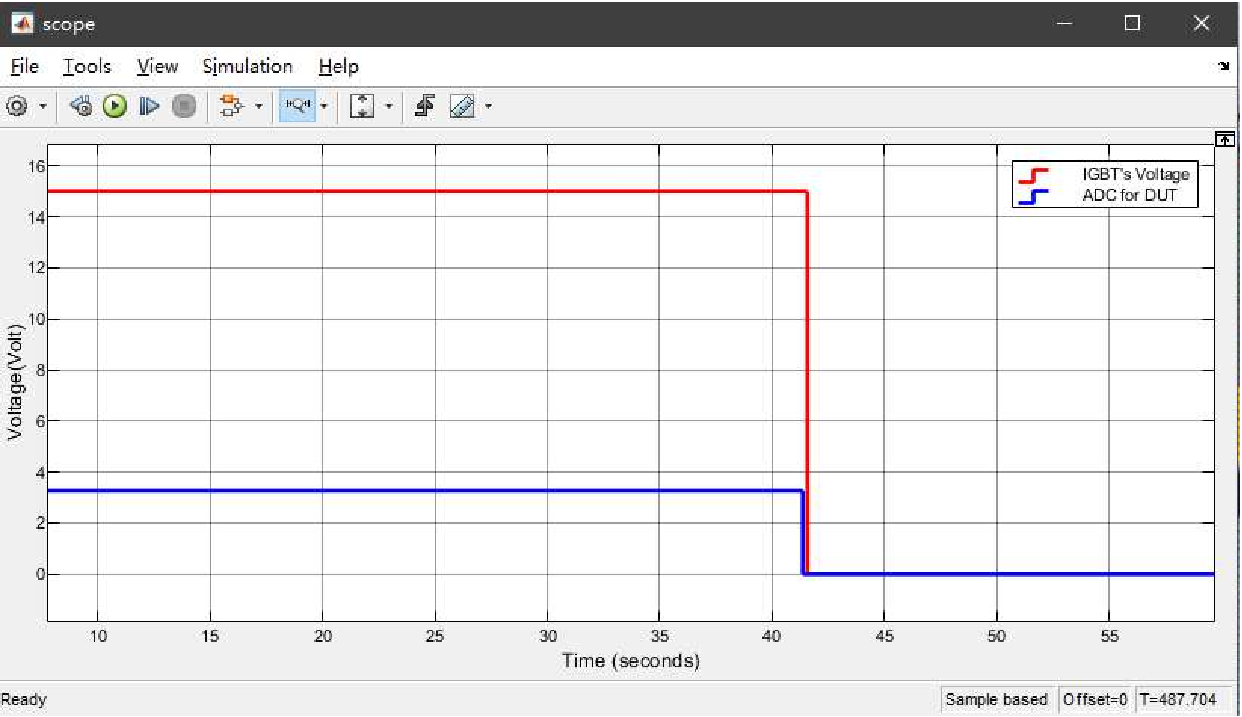
\includegraphics[width=13cm]{grafiken/3.4.pdf}
	\caption{Simulation results} 
	\label{fig:3.4}
\end{figure}
\FloatBarrier
The Figure~\ref{fig:3.4} above is the Simulation results.
\\


At first press the Pushbutton($S_{1}$), the IGBT gate voltage is 15V, the voltage across the tested unit is 3.5V, then release the button, because the circuit is a self-locking circuit, the IGBT gate voltage is provided by the output voltage of the comparator. At this time, the gate voltage of the IGBT and the voltage across DUT are unchanged. In about 42s, the external voltage is manually(change the switch($S_{2}$) applied to the GaN MOSFET. At this time, the GaN MOSFET enters the saturation mode, and the voltage across the tested cell drops to 0V rapidly. After comparing with the comparator, the time is about 1.5 microseconds, the IGBT The gate voltage is reduced to 0V, and the IGBT is quickly turned off, thereby protecting the component under test.
\\
The voltage output result is a little choppy because of LM393’s circuit property. In actual design, the filter capacitor is added to LM393. 

\chapter{Design of the measuring system}
\label{chap:Design of the measuring system}
% 4
In order to measure multiple voltage signals and temperature signals at the same time, this chapter uses two different microcontrollers to work with the network module W5500 and the temperature sensor DS18b20 for data measurement.
\\

\section{Approximate structure of the system}
\label{sec:Approximate structure of the system}
% 4.1

\begin{figure}[!ht]
	\centering
	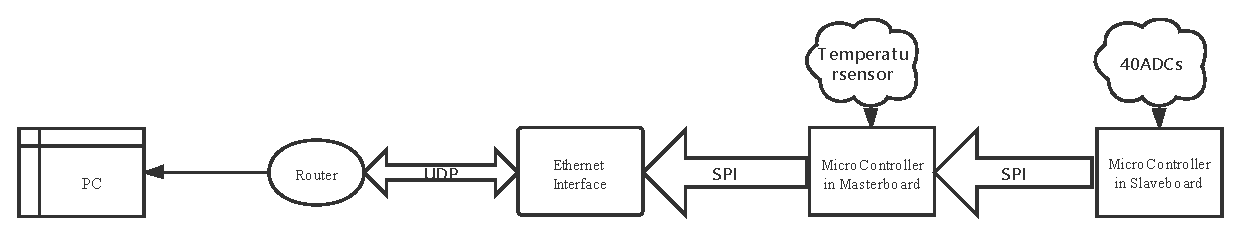
\includegraphics[width=15cm]{grafiken/4.1.eps}
	\caption{Measurement hardware circuit overview} 
	\label{fig:4.1}
\end{figure}
\FloatBarrier
As shown in the Figure~\ref{fig:4.1} above, two different microcontrollers are used to collect and transmit signals respectively. At the same time, the microcontroller on the motherboard also needs to collect temperature signals and communicate with the Ethernet chip W5500 through the SPI protocol. The collected signal is transferred to the PC.
In this circuit, the mature SCM chip STM32F429ZG of ST Company is used as the Ethernet-host connection chip. Since STM32F429 has more than 6-line SPI channels, it can be used as the chip to link with various chips. Since each STM32F303ZET6 has more than 40-channel ADC with the high cost performance, STM32F303ZET6 is used as the voltage signal chip for acquisition. 
The specific circuit diagram is shown below: 

\begin{figure}[!ht]
	\centering
	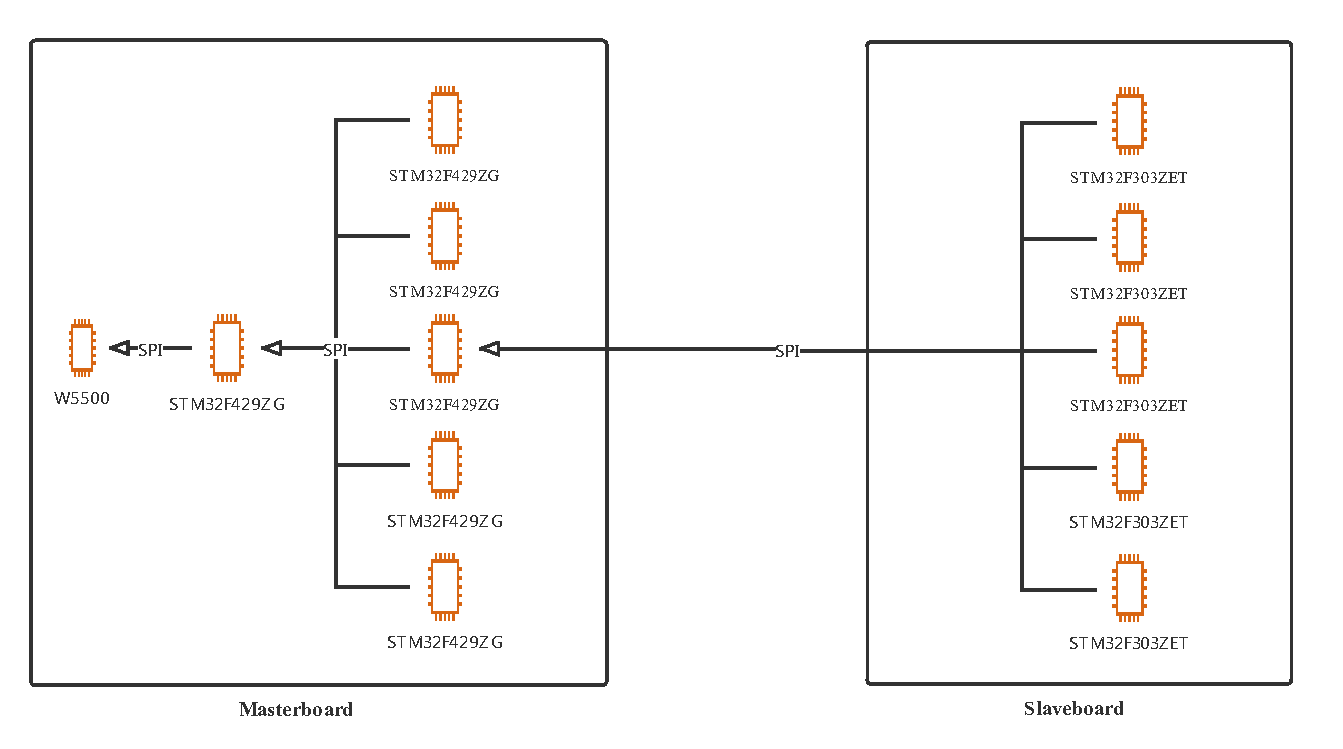
\includegraphics[width=15cm]{grafiken/4.2.pdf}
	\caption{Masterboard and Slaveboard hardware circuit overview} 
	\label{fig:4.2}
\end{figure}
\FloatBarrier

\section{Calculation of necessary number of channels/STM32}
\label{sec:Calculation of necessary number of channels/STM32}
% 4.2
If we measure 1000 units under test and each STM32F303ZET provides 40
independent ADCs, we need 1000/40=25 STM32F303 chips. The following
table~\ref{tab:4.1} shows the independent ADC distribution of each stm32F303:

% Please add the following required packages to your document preamble:
% \usepackage{booktabs}
% \usepackage[table,xcdraw]{xcolor}
% If you use beamer only pass "xcolor=table" option, i.e. \documentclass[xcolor=table]{beamer}
\begin{table}[]
\begin{tabular}{@{}lllll@{}}
\toprule
\rowcolor[HTML]{EFEFEF} 
Quantity & PINs & ADC1 channelnumber & PINs & ADC2 channelnumber \\ \midrule
\multicolumn{1}{|l|}{\cellcolor[HTML]{EFEFEF}1} & \multicolumn{1}{l|}{PA0} & \multicolumn{1}{l|}{ADC1 IN1} & \multicolumn{1}{l|}{PA4} & \multicolumn{1}{l|}{ADC2 IN1} \\ \midrule
\multicolumn{1}{|l|}{\cellcolor[HTML]{EFEFEF}2} & \multicolumn{1}{l|}{PA1} & \multicolumn{1}{l|}{ADC1 IN2} & \multicolumn{1}{l|}{PA5} & \multicolumn{1}{l|}{ADC2 IN2} \\ \midrule
\multicolumn{1}{|l|}{\cellcolor[HTML]{EFEFEF}3} & \multicolumn{1}{l|}{PA2} & \multicolumn{1}{l|}{ADC1 IN3} & \multicolumn{1}{l|}{PA6} & \multicolumn{1}{l|}{ADC2 IN3} \\ \midrule
\multicolumn{1}{|l|}{\cellcolor[HTML]{EFEFEF}4} & \multicolumn{1}{l|}{PA3} & \multicolumn{1}{l|}{ADC1 IN4} & \multicolumn{1}{l|}{PA7} & \multicolumn{1}{l|}{ADC2 IN4} \\ \midrule
\multicolumn{1}{|l|}{\cellcolor[HTML]{EFEFEF}5} & \multicolumn{1}{l|}{PB11} & \multicolumn{1}{l|}{ADC1 IN14} & \multicolumn{1}{l|}{PB2} & \multicolumn{1}{l|}{ADC2 IN12} \\ \midrule
\multicolumn{1}{|l|}{\cellcolor[HTML]{EFEFEF}6} & \multicolumn{1}{l|}{PC0} & \multicolumn{1}{l|}{ADC1 IN6} & \multicolumn{1}{l|}{PC4} & \multicolumn{1}{l|}{ADC2 IN5} \\ \midrule
\multicolumn{1}{|l|}{\cellcolor[HTML]{EFEFEF}7} & \multicolumn{1}{l|}{PC1} & \multicolumn{1}{l|}{ADC1 IN7} & \multicolumn{1}{l|}{PC5} & \multicolumn{1}{l|}{ADC2 IN11} \\ \midrule
\multicolumn{1}{|l|}{\cellcolor[HTML]{EFEFEF}8} & \multicolumn{1}{l|}{PC2} & \multicolumn{1}{l|}{ADC1 IN8} & \multicolumn{1}{l|}{} & \multicolumn{1}{l|}{} \\ \midrule
\multicolumn{1}{|l|}{\cellcolor[HTML]{EFEFEF}9} & \multicolumn{1}{l|}{PC3} & \multicolumn{1}{l|}{ADC1 IN9} & \multicolumn{1}{l|}{} & \multicolumn{1}{l|}{} \\ \midrule
\multicolumn{1}{|l|}{\cellcolor[HTML]{EFEFEF}10} & \multicolumn{1}{l|}{PF2} & \multicolumn{1}{l|}{ADC1 IN10} & \multicolumn{1}{l|}{} & \multicolumn{1}{l|}{} \\ \midrule
\multicolumn{1}{|l|}{\cellcolor[HTML]{EFEFEF}11} & \multicolumn{1}{l|}{PF4} & \multicolumn{1}{l|}{ADC1 IN5} & \multicolumn{1}{l|}{} & \multicolumn{1}{l|}{} \\ \midrule
\multicolumn{1}{|l|}{\cellcolor[HTML]{EFEFEF}12} & \multicolumn{1}{l|}{} & \multicolumn{1}{l|}{} & \multicolumn{1}{l|}{} & \multicolumn{1}{l|}{} \\ \midrule
\multicolumn{1}{|l|}{\cellcolor[HTML]{EFEFEF}13} & \multicolumn{1}{l|}{} & \multicolumn{1}{l|}{} & \multicolumn{1}{l|}{} & \multicolumn{1}{l|}{} \\ \midrule
\multicolumn{1}{|l|}{\cellcolor[HTML]{EFEFEF}14} & \multicolumn{1}{l|}{} & \multicolumn{1}{l|}{} & \multicolumn{1}{l|}{} & \multicolumn{1}{l|}{} \\ \midrule
\multicolumn{1}{|l|}{\cellcolor[HTML]{EFEFEF}15} & \multicolumn{1}{l|}{} & \multicolumn{1}{l|}{} & \multicolumn{1}{l|}{} & \multicolumn{1}{l|}{} \\ \midrule
\rowcolor[HTML]{EFEFEF} 
\multicolumn{1}{|l|}{\cellcolor[HTML]{EFEFEF}Summe} & \multicolumn{1}{l|}{\cellcolor[HTML]{EFEFEF}} & \multicolumn{1}{l|}{\cellcolor[HTML]{EFEFEF}11} & \multicolumn{1}{l|}{\cellcolor[HTML]{EFEFEF}} & \multicolumn{1}{l|}{\cellcolor[HTML]{EFEFEF}7} \\ \midrule
 &  &  &  &  \\ \midrule
\rowcolor[HTML]{EFEFEF} 
\multicolumn{1}{|l|}{\cellcolor[HTML]{EFEFEF}Quantity} & \multicolumn{1}{l|}{\cellcolor[HTML]{EFEFEF}PINs} & \multicolumn{1}{l|}{\cellcolor[HTML]{EFEFEF}ADC3 channelnumber} & \multicolumn{1}{l|}{\cellcolor[HTML]{EFEFEF}PINs} & \multicolumn{1}{l|}{\cellcolor[HTML]{EFEFEF}ADC4 channelnumber} \\ \midrule
\multicolumn{1}{|l|}{\cellcolor[HTML]{EFEFEF}1} & \multicolumn{1}{l|}{PB0} & \multicolumn{1}{l|}{ADC3 IN12} & \multicolumn{1}{l|}{PB12} & \multicolumn{1}{l|}{ADC4 IN3} \\ \midrule
\multicolumn{1}{|l|}{\cellcolor[HTML]{EFEFEF}2} & \multicolumn{1}{l|}{PB1} & \multicolumn{1}{l|}{ADC3 IN1} & \multicolumn{1}{l|}{PB14} & \multicolumn{1}{l|}{ADC4 IN4} \\ \midrule
\multicolumn{1}{|l|}{\cellcolor[HTML]{EFEFEF}3} & \multicolumn{1}{l|}{PB13} & \multicolumn{1}{l|}{ADC3 IN5} & \multicolumn{1}{l|}{PB15} & \multicolumn{1}{l|}{ADC4 IN5} \\ \midrule
\multicolumn{1}{|l|}{\cellcolor[HTML]{EFEFEF}4} & \multicolumn{1}{l|}{PD10} & \multicolumn{1}{l|}{ADC3 IN7} & \multicolumn{1}{l|}{PD8} & \multicolumn{1}{l|}{ADC4 IN12} \\ \midrule
\multicolumn{1}{|l|}{\cellcolor[HTML]{EFEFEF}5} & \multicolumn{1}{l|}{PD11} & \multicolumn{1}{l|}{ADC3 IN8} & \multicolumn{1}{l|}{PD9} & \multicolumn{1}{l|}{ADC4 IN13} \\ \midrule
\multicolumn{1}{|l|}{\cellcolor[HTML]{EFEFEF}6} & \multicolumn{1}{l|}{PD12} & \multicolumn{1}{l|}{ADC3 IN9} & \multicolumn{1}{l|}{PE14} & \multicolumn{1}{l|}{ADC4 IN1} \\ \midrule
\multicolumn{1}{|l|}{\cellcolor[HTML]{EFEFEF}7} & \multicolumn{1}{l|}{PD13} & \multicolumn{1}{l|}{ADC3 IN10} & \multicolumn{1}{l|}{PE15} & \multicolumn{1}{l|}{ADC4 IN2} \\ \midrule
\multicolumn{1}{|l|}{\cellcolor[HTML]{EFEFEF}8} & \multicolumn{1}{l|}{PD14} & \multicolumn{1}{l|}{ADC3 IN11} & \multicolumn{1}{l|}{} & \multicolumn{1}{l|}{} \\ \midrule
\multicolumn{1}{|l|}{\cellcolor[HTML]{EFEFEF}9} & \multicolumn{1}{l|}{PE7} & \multicolumn{1}{l|}{ADC3 IN13} & \multicolumn{1}{l|}{} & \multicolumn{1}{l|}{} \\ \midrule
\multicolumn{1}{|l|}{\cellcolor[HTML]{EFEFEF}10} & \multicolumn{1}{l|}{PE8} & \multicolumn{1}{l|}{ADC3 IN6} & \multicolumn{1}{l|}{} & \multicolumn{1}{l|}{} \\ \midrule
\multicolumn{1}{|l|}{\cellcolor[HTML]{EFEFEF}11} & \multicolumn{1}{l|}{PE9} & \multicolumn{1}{l|}{ADC3 IN2} & \multicolumn{1}{l|}{} & \multicolumn{1}{l|}{} \\ \midrule
\multicolumn{1}{|l|}{\cellcolor[HTML]{EFEFEF}12} & \multicolumn{1}{l|}{PE10} & \multicolumn{1}{l|}{ADC3 IN14} & \multicolumn{1}{l|}{} & \multicolumn{1}{l|}{} \\ \midrule
\multicolumn{1}{|l|}{\cellcolor[HTML]{EFEFEF}13} & \multicolumn{1}{l|}{PE11} & \multicolumn{1}{l|}{ADC3 IN15} & \multicolumn{1}{l|}{} & \multicolumn{1}{l|}{} \\ \midrule
\multicolumn{1}{|l|}{\cellcolor[HTML]{EFEFEF}14} & \multicolumn{1}{l|}{PE12} & \multicolumn{1}{l|}{ADC3 IN16} & \multicolumn{1}{l|}{} & \multicolumn{1}{l|}{} \\ \midrule
\multicolumn{1}{|l|}{\cellcolor[HTML]{EFEFEF}15} & \multicolumn{1}{l|}{PE13} & \multicolumn{1}{l|}{ADC3 IN3} & \multicolumn{1}{l|}{} & \multicolumn{1}{l|}{} \\ \midrule
\rowcolor[HTML]{EFEFEF} 
Summe &  & 15 &  & 7 \\ \bottomrule
 
\end{tabular}
	\caption{List of ADC channels used}
	\label{tab:4.1}
\end{table}

To measure 1000 DUT components, at least 1000 lines of ADC should be used. To ensure signal quality, electromagnetic compatibility, and developmental cost, ADC is only used on the slaveboard, as shown in the Figure below~\ref{fig:4.3}: 

% At the same time, you need to configure the pins of stm32F303ZET in the
% development environment, and the results are shown in the following Figure~\ref{fig:4.3}:
% Figure~\ref{fig:4.3}
\begin{figure}[!ht]
	\centering
	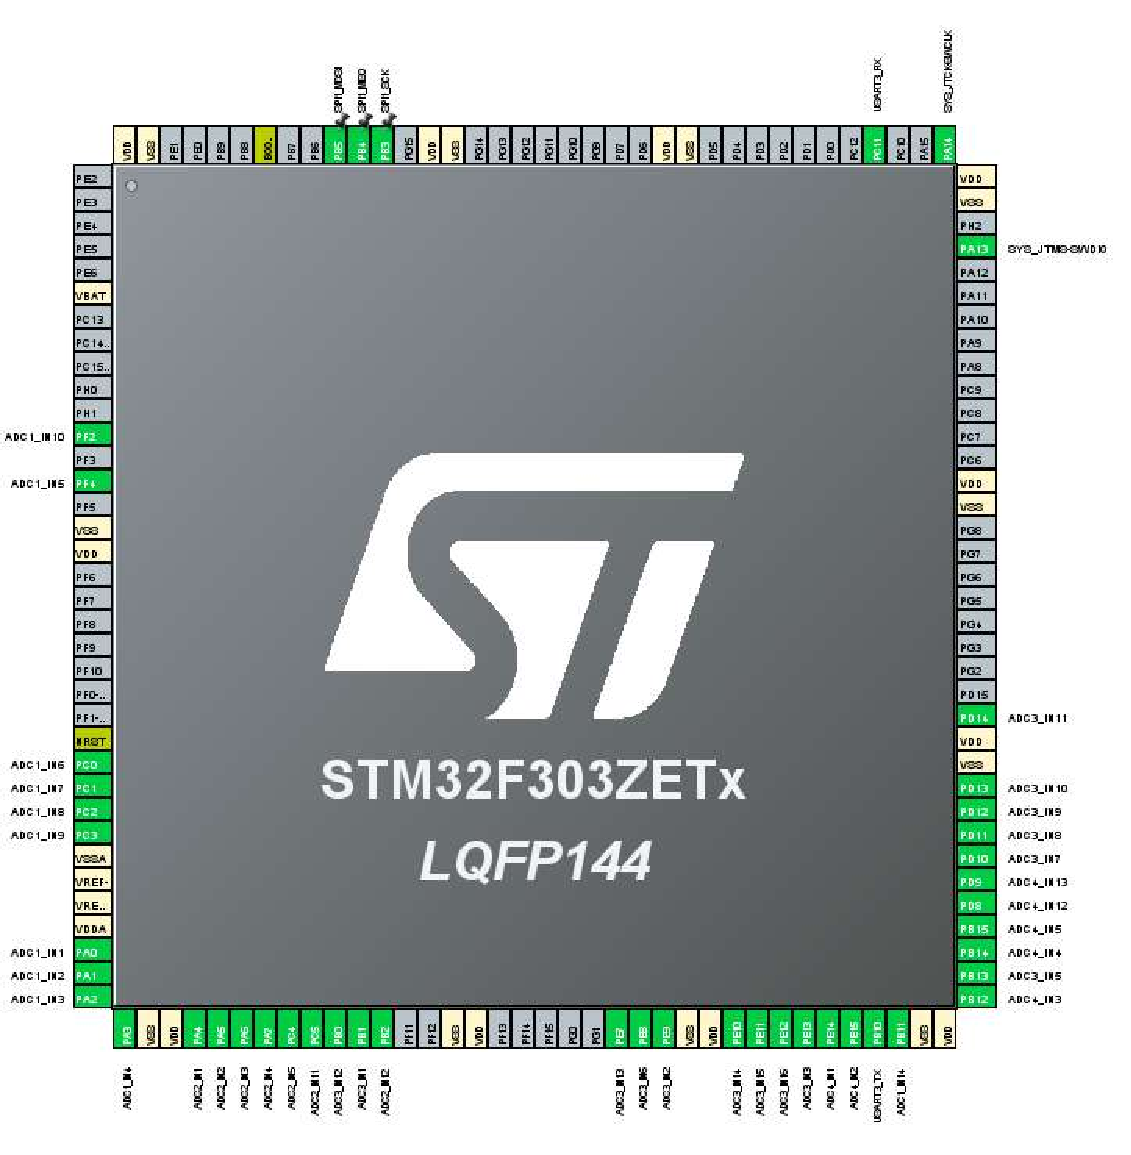
\includegraphics[width=15cm]{grafiken/4.3.pdf}
	\caption{ADC Channel selection of Slaveboard in CubeMX IDE} 
	\label{fig:4.3}
\end{figure}
\FloatBarrier
\\

\section{Calculation of power}
\label{sec:Calculation of power}
% 4.3
According to STM32F429 official specification, the typical value of STM32 operating power current is 200mAH but we need to select SPI channel and GPIO interface as measurement and use multi-channel ADC for measurement. When the circuit board encounters high temperature and high pressure or improper situations, the required power will rise. Under the circumstance, we need to consider the maximum power (495mW). 
This paper calculate the masterboard’s maximum demanded power, thus:

\begin{center} 
\begin{equation}
P_{Masterboard} = \sum \left \lceil n_{component}*P_{component}\right \rceil 
\\
=1*\left \lceil P_{W5500}  \right \rceil +6* \left \lceil P_{STM32F429}  \right \rceil+ 4* \left \lceil P_{DS18b20}\right \rceil = 3370mW
\end{equation}
\end{center}
\\
Since each DCDC converter chip TWR6 can provide 6W switching power supply(which provides 350W), each masterboard only needs a DCDC convertor. 
Then calculate the slaveboard’s maximum demanded power, thus: 
\begin{center} 
\begin{equation}
P_{Slaveboard} = \sum \left \lceil n_{component}*P_{component}\right \rceil=5* \left \lceil P_{STM32F303}  \right \rceil= 2475mW
\end{equation}
\end{center}
%speed
In other words, the slaveboard only needs a DCDC converter.
% We calculate the main control mainboard’s maximum demanded power by ourselves, thus: 

\chapter{Detailed presentation of the measuring system}
\label{chap:Detailed presentation of the measuring system}
% 5
In order to design the measurement system, the hardware part should be designed first, so as to better evaluate the software requirements. When designing the software part, try to make the entire measurement system more accurate and more suitable for long-term use.

\section{Hardware}
\label{sec:Hardware}
% 5.1
The hardware design is divided into three parts: the spatial distribution of the temperature sensor and the motherboard and the selection of the control shielding wire.
\subsection{Temperature Sensor}
\label{sec:Temperature Sensor}
% 5.1.1
Since we have determined the ADC selection, temperature changes will also
have an impact on GaN.
At this time, we should choose a temperature sensor to measure the outside
of the component under test.
DS18B20 is a commonly used digital temperature sensor. Its output is a digital
signal. It has the characteristics of small size, low hardware overhead, strong
anti-interference ability, and high precision. DS18B20 digital temperature
sensor is easy to wire, and can be used in many occasions after being
packaged, such as pipeline type, threaded type, magnet adsorption type,
stainless steel package type, and various models, such as LTM8877, LTM8874
and so on.
The DS18b20 sensor is a single-bus transmission signal. The connection
method between it and the microcontroller is shown in the Figure below:

% Figure~\ref{fig:4.3}
\begin{figure}[!ht]
	\centering
	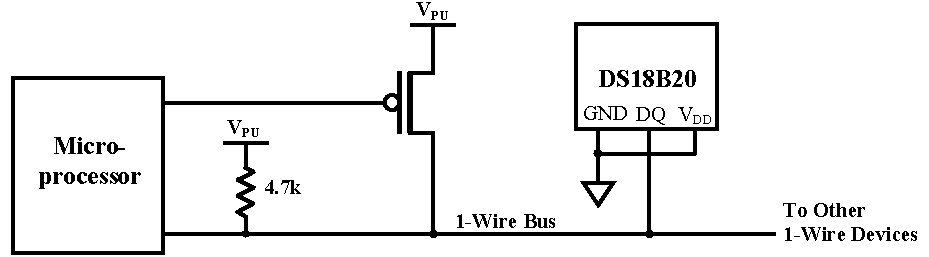
\includegraphics[width=15cm]{grafiken/5.1.pdf}
	\caption{ADC Channel selection of Slaveboard in CubeMX IDE} 
	\label{fig:5.1}
\end{figure}
\FloatBarrier
\\
Mainly change its appearance according to different applications. The packaged DS18B20 can be used for cable trench temperature measurement, blast furnace water circulation temperature measurement, boiler temperature measurement, machine room temperature measurement, agricultural greenhouse temperature measurement, clean room temperature measurement, ammunition warehouse temperature measurement and other non-limiting temperature occasions. Wear-resistant and anti-collision, small size, easy to use, various packaging forms, suitable for various small space equipment digital temperature measurement and control fields.

\subsection{The spatial distribution of the boards}
\label{sec:The spatial distribution of the boards}
% 5.1.2
Since the length and width of each circuit board are 150mm and 100mm, so the neutral board has enough space to put all six measuring boards. The following Figures show the spatial distribution of boards on the neutral board:
\begin{figure}[!ht]
	\centering
	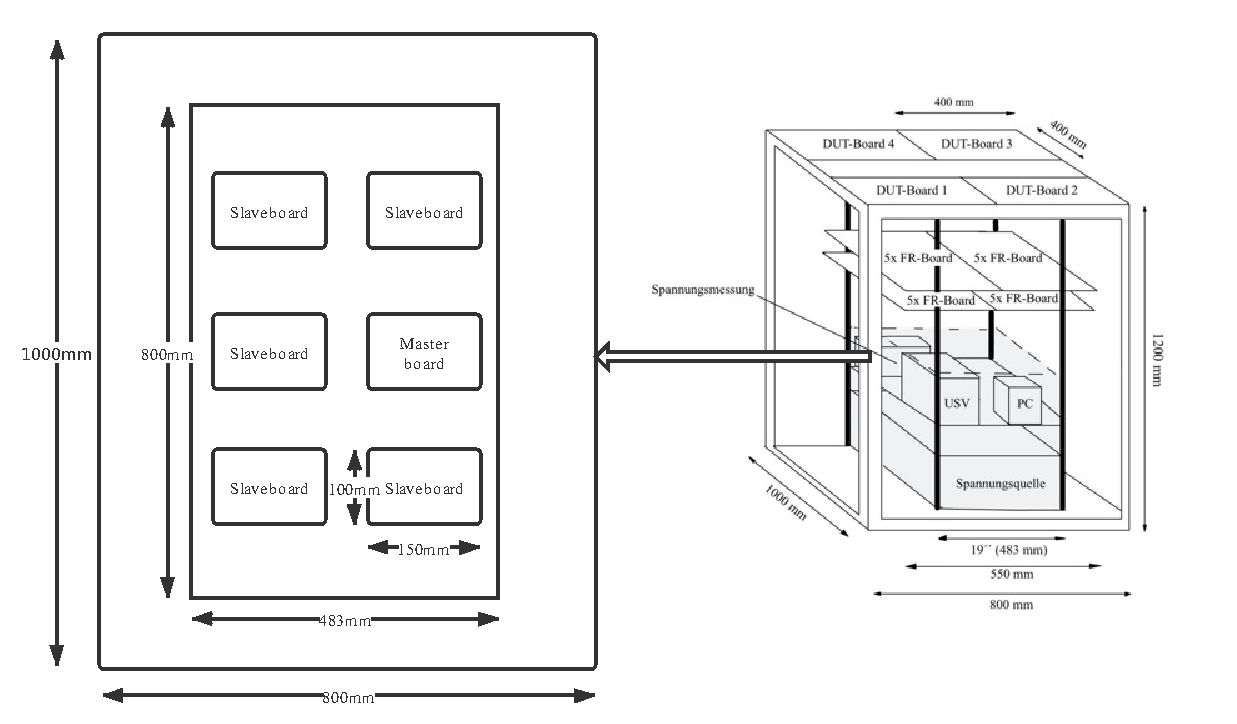
\includegraphics[width=16cm]{grafiken/5.2.pdf}
	\caption{Spatial distribution of boards(2D)} 
	\label{fig:5.2}
\end{figure}
\FloatBarrier
\\

\begin{figure}[!ht]
	\centering
	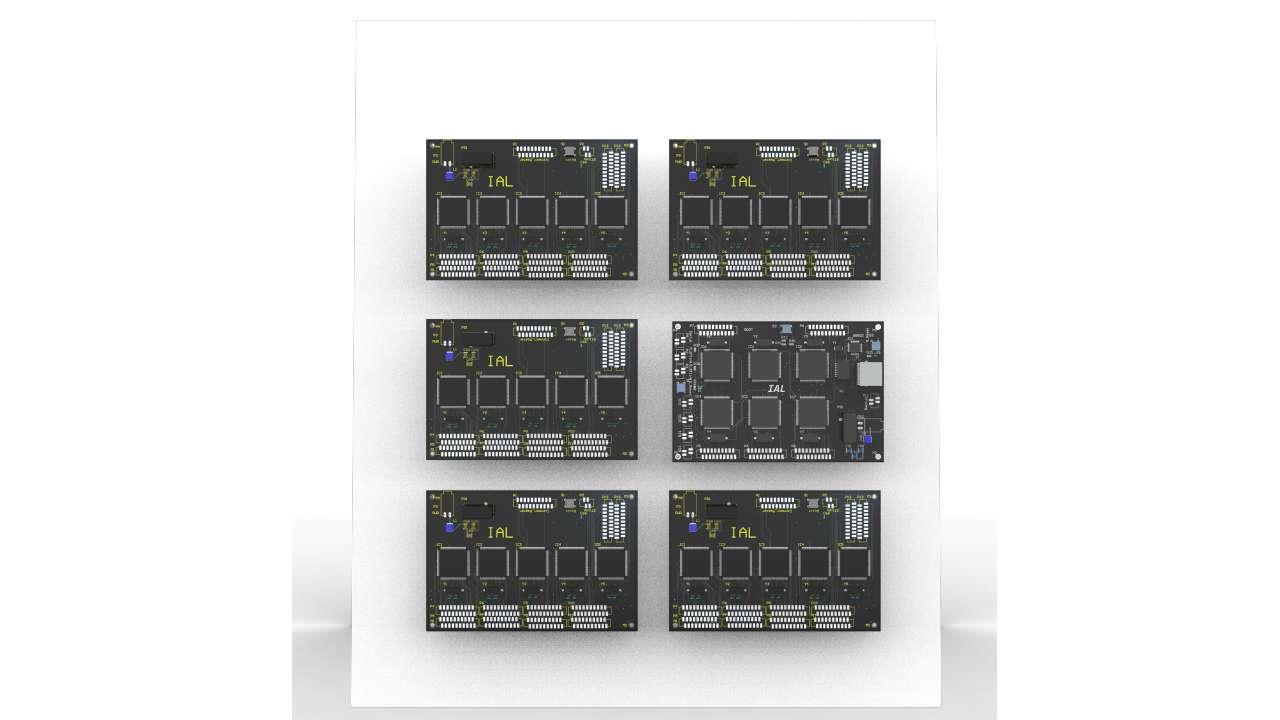
\includegraphics[width=16cm]{grafiken/5.3.pdf}
	\caption{Spatial distribution of boards(3D)} 
	\label{fig:5.3}
\end{figure}
\FloatBarrier




\subsection{Control shielding wire}
\label{sec:Control shielding wire}
% 5.1.3
In order to have good electrical conductivity and prevent electromagnetic interference, this article compares several widely used CY cables, SY cables, YY cables and LiYCY and LiYY cables. These cables are designed for various industrial process automation applications, including signal transmission, measurement, Control and regulation. These control cables are usually referred to by applications, such as machine power cables, motor cables and robot cables. They are also called multi-core cables, control flexible cables and control flexible cables.
According to their structural characteristics, these flexible cables can be suitable for use under light, medium or high mechanical stress. They also provide various degrees of protection against electrical interference and resistance to corrosive substances and oils.
There are two kinds of cables that are very suitable for connecting the network(LiYCY cable) and the communication between the master board and the slave board(CY cable).
\\
CY cable (YSLCY / HSLCH) : Multicore screened flexible cable with Polyethylene Terephthalate (PETP) for electromagnetic interference free-transmission
\\
LiYCY cable: Screened and shielded cable for applications where moderate mechanical stress and electromagnetic screening is required.
The two control shielded wires from left to right in the Figure below are LiYCY and HSLCH respectively.
\\
The Figure~\ref{fig:5.4} below shows LiYCY and HSLCH from left to right. These two kinds of control shielded cables can be used as the connection line between the network cable and the master and slave respectively.
\begin{figure}[!ht]
	\centering
	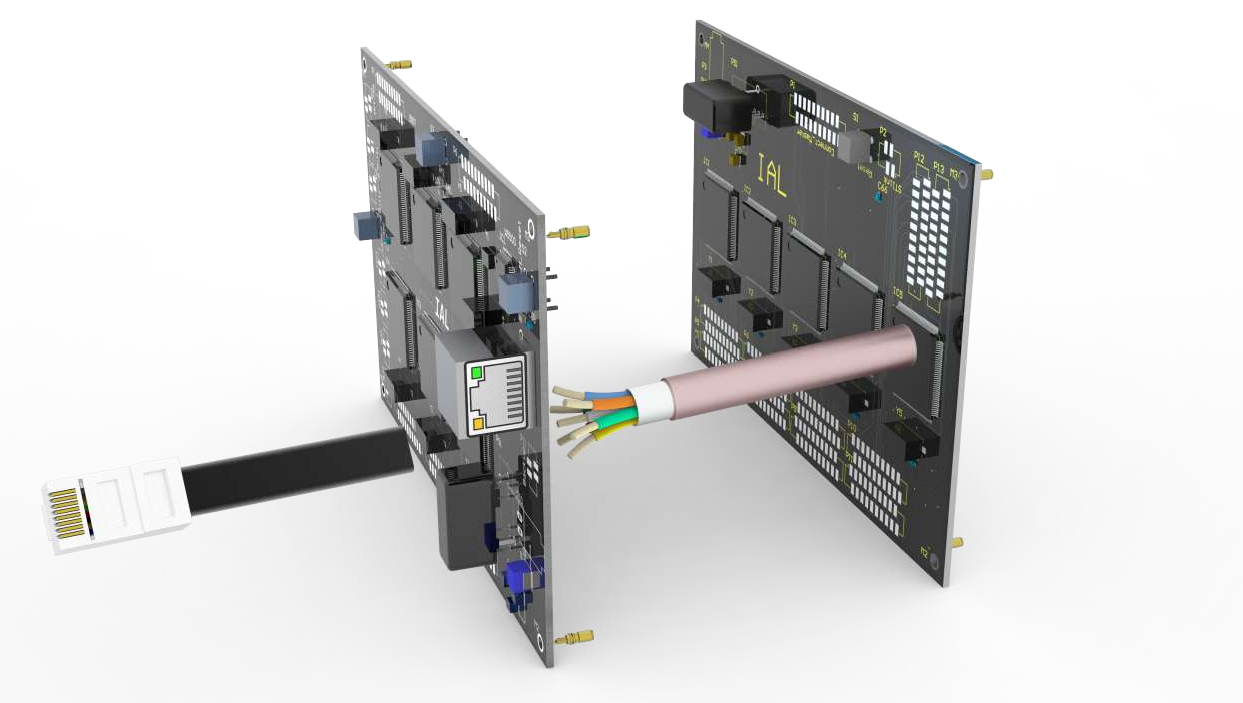
\includegraphics[width=16cm]{grafiken/5.4.pdf}
	\caption{Control shielding wire LiYCY(left) and HSLCH(right)} 
	\label{fig:5.4}
\end{figure}
\FloatBarrier
\\

\section{Software}
\label{sec:Software}
% 5.2
The software part mainly focuses on the design of acquisition speed, arithmetic average filter, debugger, front-end and back-end.

\subsection{Measurespeed}
\label{sec:Measurespeed}
% 5.2.1
In order to improve reliability and signal-to-noise ratio, this article needs to explore the upper limit of the acquisition speed to ensure that all data can be correctly sent to the PC.
First of all, we have to determine the sampling speed of the temperature sensor. Each cycle of the temperature sensor is divided into two phases: read and write, as shown in the following Figure~\ref{fig:5.5}:
\begin{figure}[!ht]
	\centering
	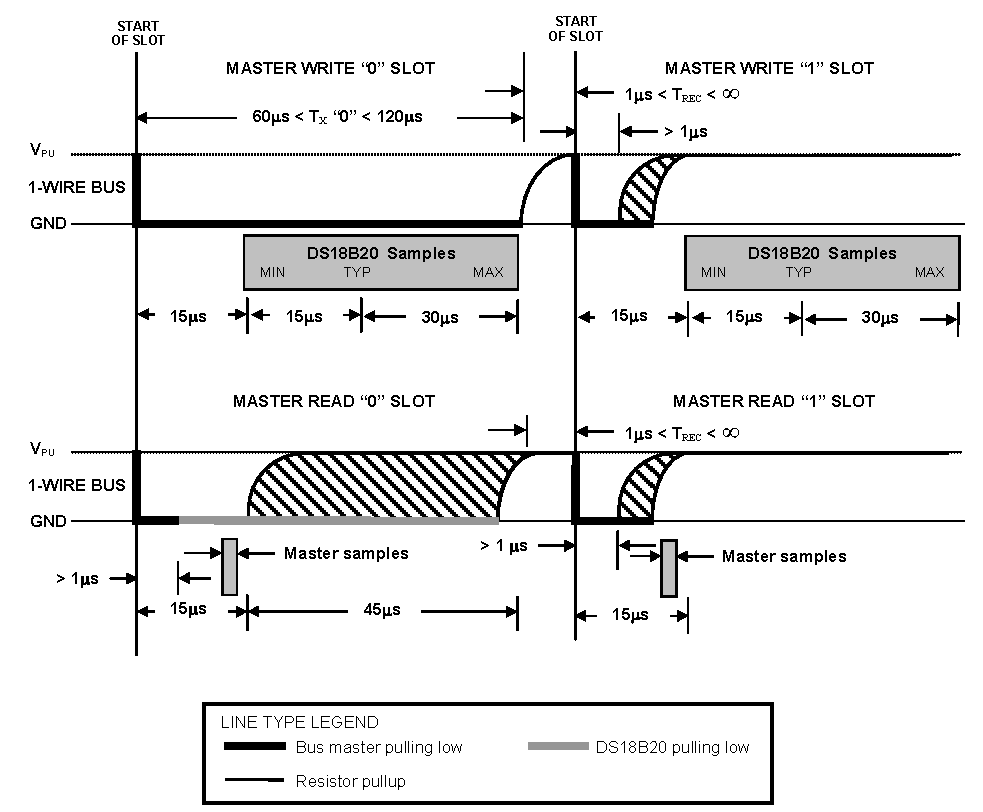
\includegraphics[width=16cm]{grafiken/5.5.pdf}
	\caption{DS18b20 write/read signal required time} 
	\label{fig:5.5}
\end{figure}
\FloatBarrier

The host writes data in DS18B20 as writing the time slot, including “0” time slot and “1” time slot. The bus host uses “1” time slot to write logic in DS18B20 and to write logic 0 in DS18B20 as writing “0” time slot. All writing time slots at least must have 60μs duration. Two adjacent writing time slots at least must have 1μs recovery time. Two writing time slots can be generated by lowering the bus through the host (see the picture below), for the sake of generating “1” time slot. 
After lowering the bus, the host must release the bus within 15μs. After releasing the bus, the pull-up resistor can recover the bus to the high level. To generate “0” time slot, after lowering the bus, the host must continue lowering the bus to satisfy the requirement of the time slot’s duration (at least 60μs). 
After the host generates the writing time slots, DS18B20 will sample the single bus(DQ) within a time quantum of 15-60μs. Within the time window of sampling, if the bus belongs to the high level, the host will write 1 in DS18B20; if the bus belongs to the low level, the host will write 0 in DS18B20. 
\\
To sum up, all writing time slots at least must have 60μs of duration. Two adjacent time slots at least must have 1μs of recovery time. All writing time slots(0 and 1) are generated by lowering the bus. 
When the host launches to read the time sequences, DS18B20 is only used to transmit data to the controller, thus the bus controller will issue the order of reading the transient memory [0xBe] or the order of reading the power mode [0xB4] and then it immediately starts reading time sequences. DS18B20 can provide the request information. Besides, the bus controller will read the time sequences after issuing the order of sending temperature conversion[0x44](or recalling EEPROM order[0xB8]) before reading time sequences. See details in the functional order in DS18B20 chip manual. 
All reading time sequences at least must reach 60μs, including two reading periods with at least 1μs recovery time. When the bus controller pulls the USB cable from the high level to the low level, as starting reading time sequences, USB cables at least must remain 1μs and then the bus is released. DS18B20 pulls up or pulls down the bus to transmit “1” or “0”. When the transmission logic “0” comes to an end, the bus will be released. When the pull-up resistor returns to the rising edge state, data from DS18B20 will be valid within 15μs after the falling edge of reading time sequences occurs. Thus, as starting reading time sequences, the bus controller must stop I/O drive into the low voltage 15μs to read I/O state. 
\\

According to the chip's specification, the slave board's SPI has only the fastest sending speed of 4MB/s, and at the same time, four slave boards need to send data to the master board. It takes at least 1.5 cycles for each ADC to collect the voltage signal, and the maximum can be set It takes 601.5 cycles. According to the manual, the conversion time is 
 
\\
\begin{center} 
\begin{equation}
max(T_{Convert}) =max(T_{Sample})+T_{Signel-convert} =601.5cyc+12.5cyc=614cyc
\end{equation}
\end{center}
\\
\begin{center} 
\begin{equation}
min(T_{Convert})=min(T_{Sample})+T_{Signel-convert} =1.5cyc+12.5cyc=14cyc
\end{equation}
\end{center}

 
Since the host main board accepts the data sent by 5 slave main boards at the same time, in order to prevent congestion, his SPI receiving speed is set to 8MB/s,
Therefore, the sending speed of each slave main board must be reduced to a sending speed of 8/5=1.6MB/s to ensure that the host main board can receive all data from the slave main board.
\\
The Figure below shows the data collection speed and data flow.
\begin{figure}[!ht]
	\centering
	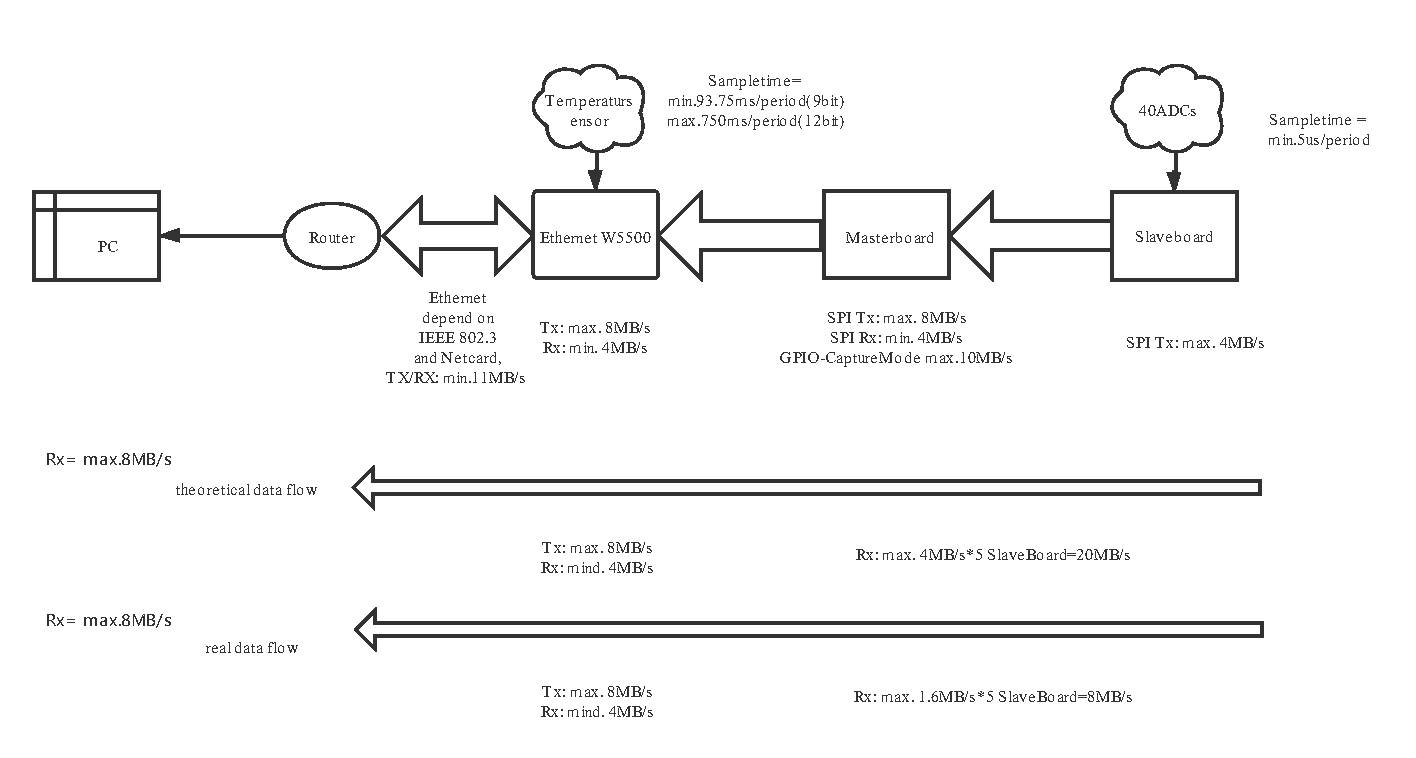
\includegraphics[width=16cm]{grafiken/5.6.pdf}
	\caption{Data collection speed and data flow} 
	\label{fig:5.6}
\end{figure}
\FloatBarrier

\\
That is to say, each time the slave board main board adopts the average filtering method cycle, a delay program must be added to ensure that each value received by the master is valid and reliable.
Since apply the mean filter method, sampling per 10 times can be used as a group of data and then through geometric mean, at least 10us is needed for sampling. 
Considering that the host mainboard accepts the data sent from 5 slave mainboards simultaneously, the SPI receiving speed is set up as 8MB/s, for the sake of preventing congestion. 
Thus, sending speed of each slave mainboard must be reduced to 1.6Mbps, for the sake of ensuring that the host mainboard can receive all data from the slaveboard. 
In other words, the slaveboard applies the mean filtering circulation to increase the delay procedure every time, so as to ensure that each value received by the host is valid and reliable. 

\subsection{Arithmetic average filter}
\label{sec:Arithmetic average filter}
% 5.2.2

In this article we will use the average filtering method to set the ADC to become a continuous acquisition and observation mode. At this point, the data received from DMA is stored in the register, and each ADC total channel completes 10 acquisition cycles then receives 10 times the channel. The data is arithmetic averaged to obtain the final sample.

\subsection{Debugger, front-end and back-end}
\label{sec:Debugger, front-end and back-end}
% 5.2.3

In order to meet the needs of the Internet of Things, the software part is structured as shown in the Figure below:
\begin{figure}[!ht]
	\centering
	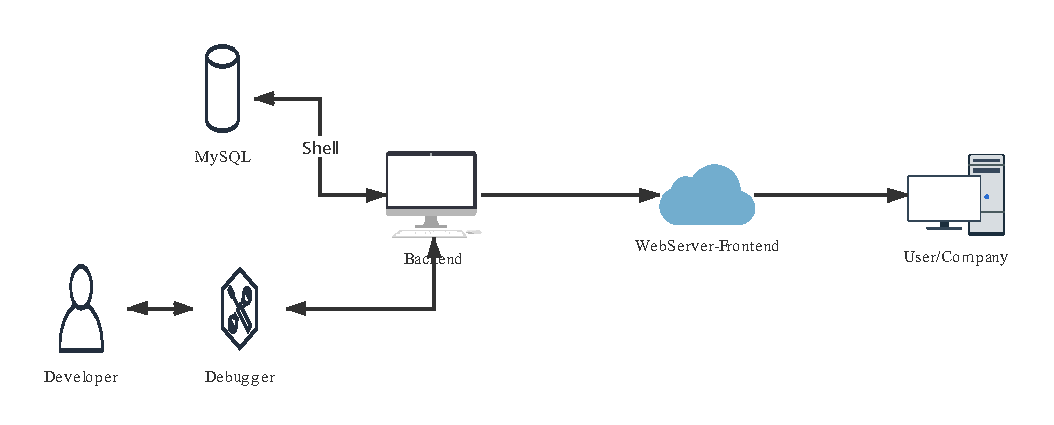
\includegraphics[width=16cm]{grafiken/5.7.pdf}
	\caption{Structure of LoT-software} 
	\label{fig:5.7}
\end{figure}
\FloatBarrier



For researchers, this article mainly uses the open source project ScriptCommunicator as a debugger. At the same time, because ScriptCommunicator does not have a continuous debugging function, a script was written in QT and C++ for continuous debugging.
The following Figure~\ref{fig:5.8} is the interface of the debugger:

\begin{figure}[!ht]
	\centering
	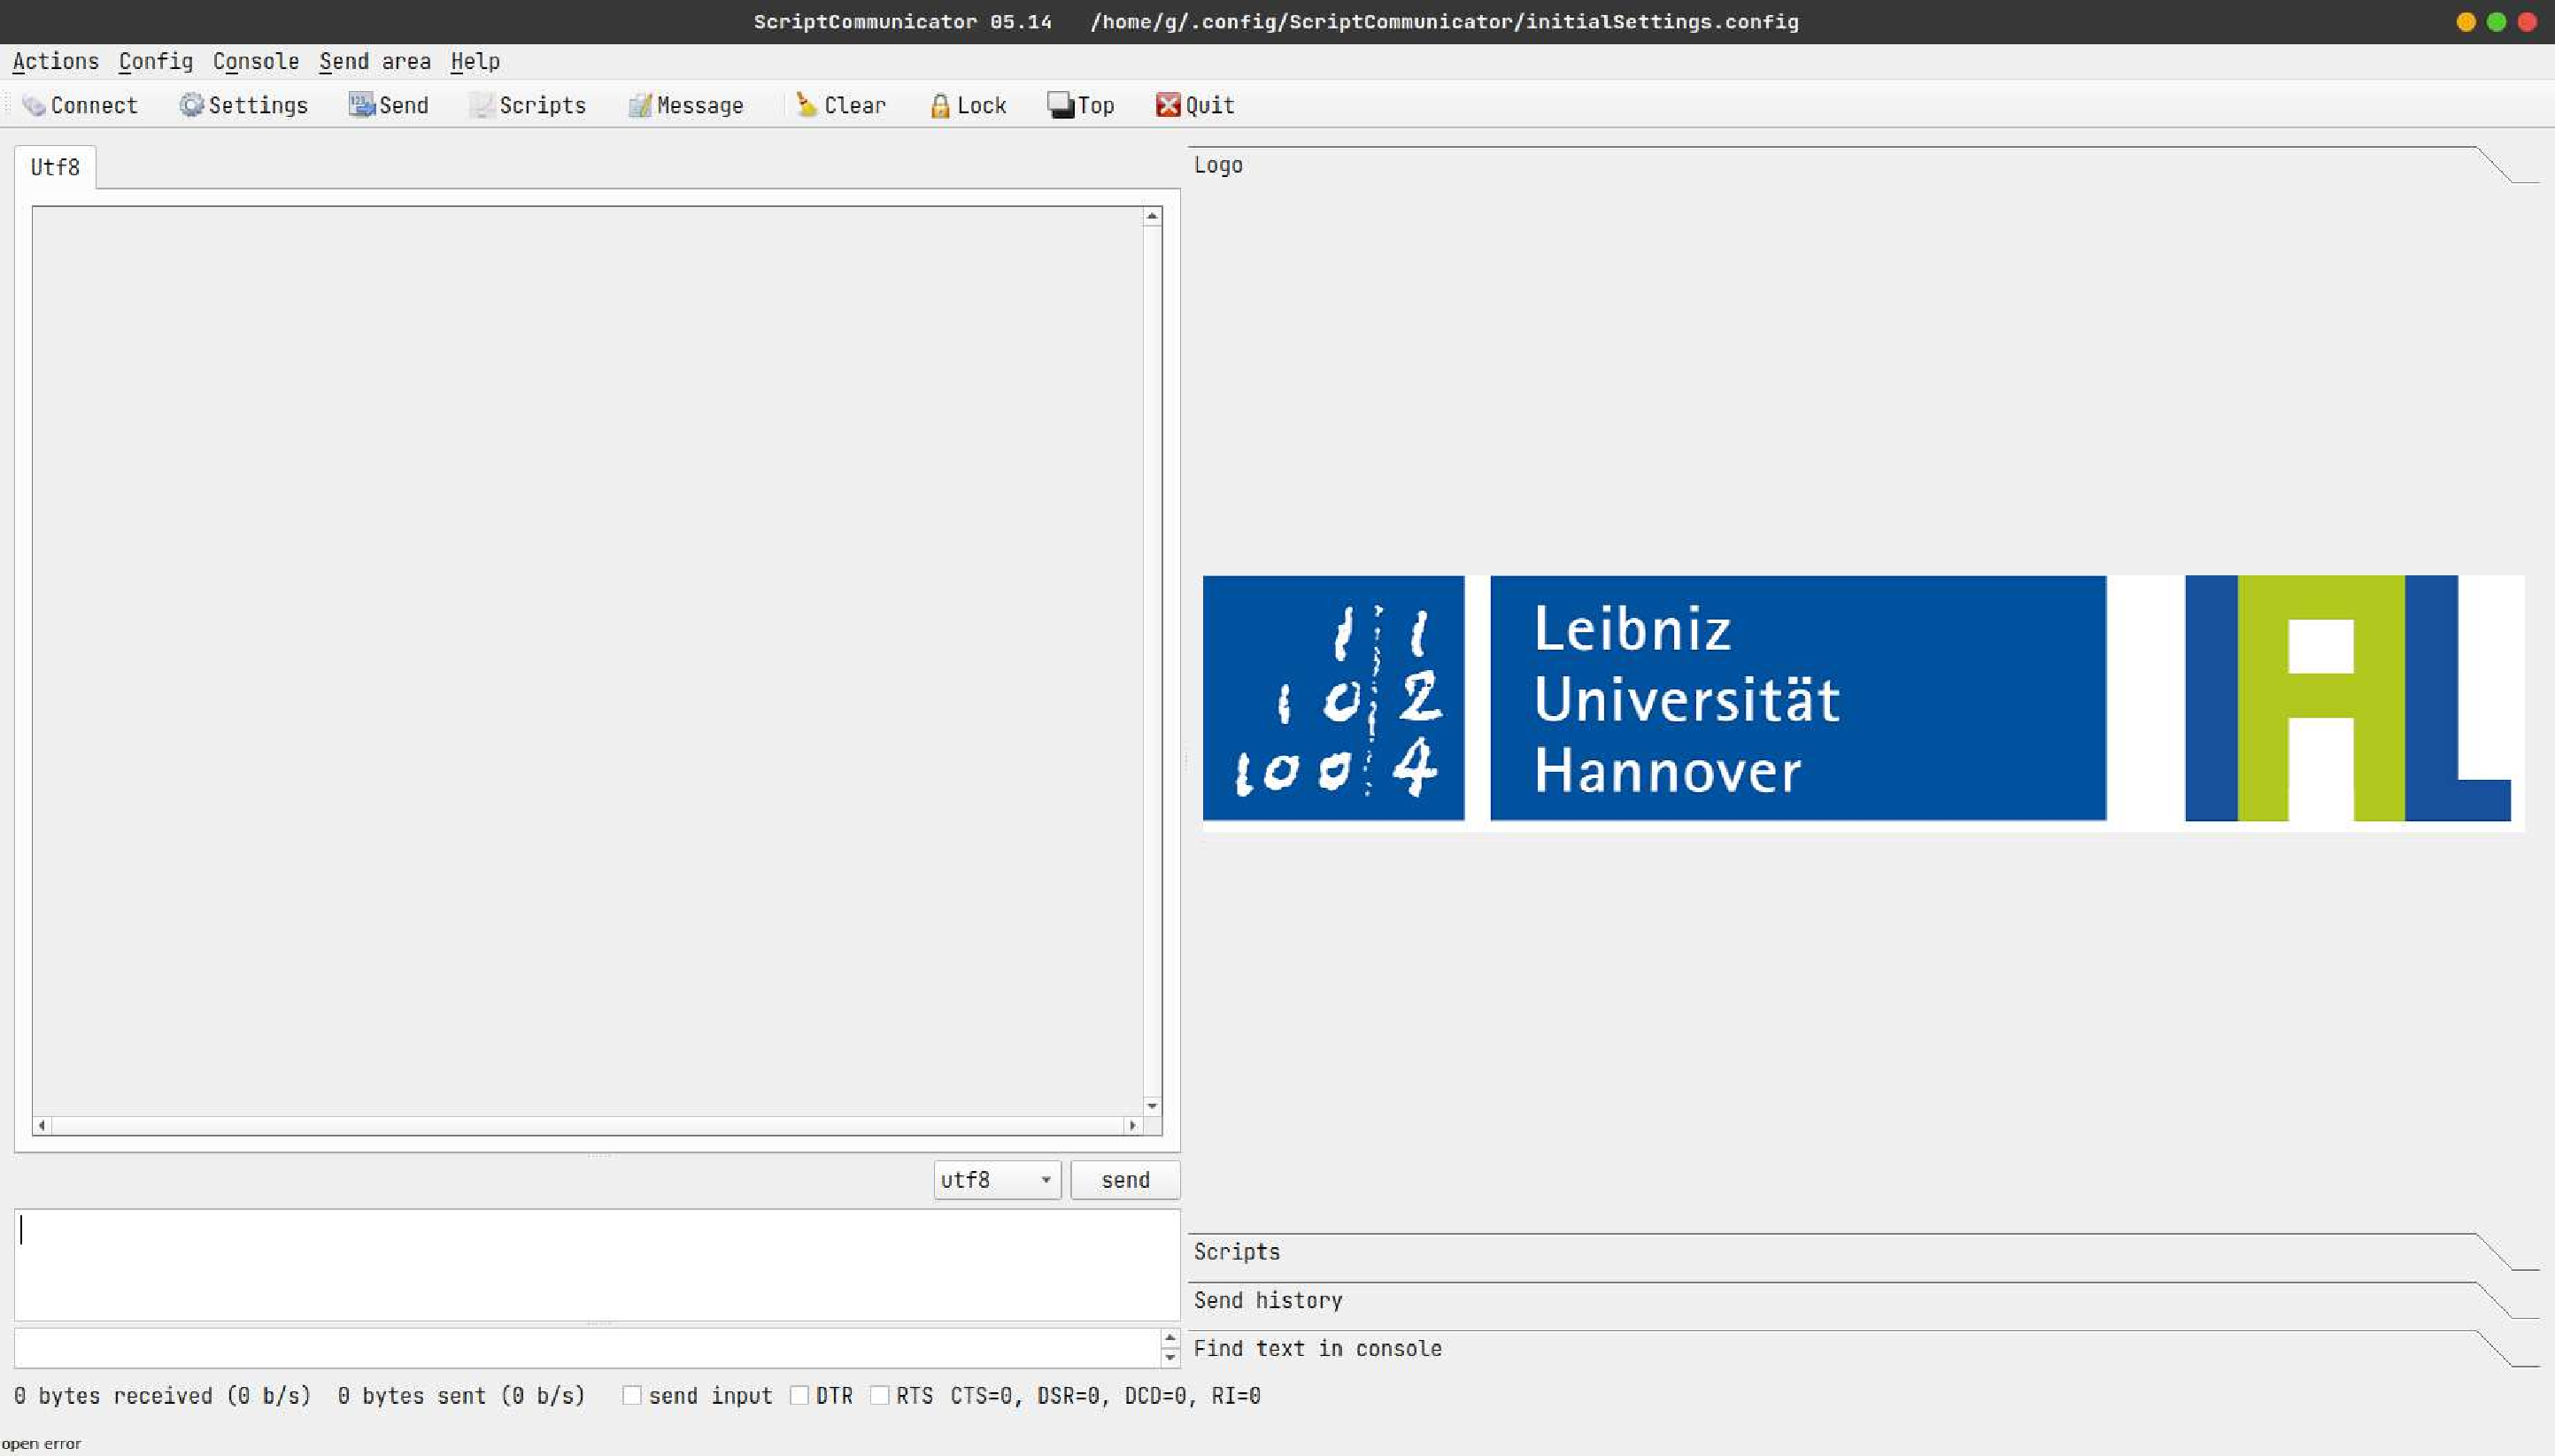
\includegraphics[width=16cm]{grafiken/5.8.pdf}
	\caption{Debugger:ScriptCommunicator} 
	\label{fig:5.8}
\end{figure}
\FloatBarrier
\\
Front end and back end:
Since Ubuntu is used as the operating system, shell scripts and netcat tools can be used to collect data from UDP and synchronize to the MySQL database. At the same time, use Springboot to build the backend, namely JavaWeb, and use MybatisPlus to construct instances and interfaces, and add a key"creat time" of the attribute data.


The GUI(Graphical user interface) that separates the front and back ends specifically refers to the browser (or client) side. One of the most misunderstood concepts for novice server-
side Java users is that JSP is a front-end technology. JSP needs to know the full name: Java Server Page. It runs in the servlet container on the server-side JVM, but the result of runningis HTML that is responsive to the browser. Servlet, the first from Java EE, already had ASPat this point (also knows the meaning of Active Server Page). Due to the need to put a lot of HTML code in servlet, the Java specification learned ASP and suggested JSP. Servlet is Java code mixed with HTML, JSP is HTML code mixed with Java. The browser doesn’t care if the server is JSP, ASP, PHP or the original servlet or HTML on the static server as long as it returns valid HTML code. So take out the static HTML part of the JSP, convert it to a simple
HTML file and put it on the HTTP server. The browser just needs to fetch the HTML code. The dynamic data part is fetched by AJAX from the server side using JS in HTML and then the dom is operated dynamically to complete the display of the dynamic content. In this way, the leading and trailing ends are separated.
The following Figure~\ref{fig:5.9}  is the homepage of the front-end:



\begin{figure}[!ht]
	\centering
	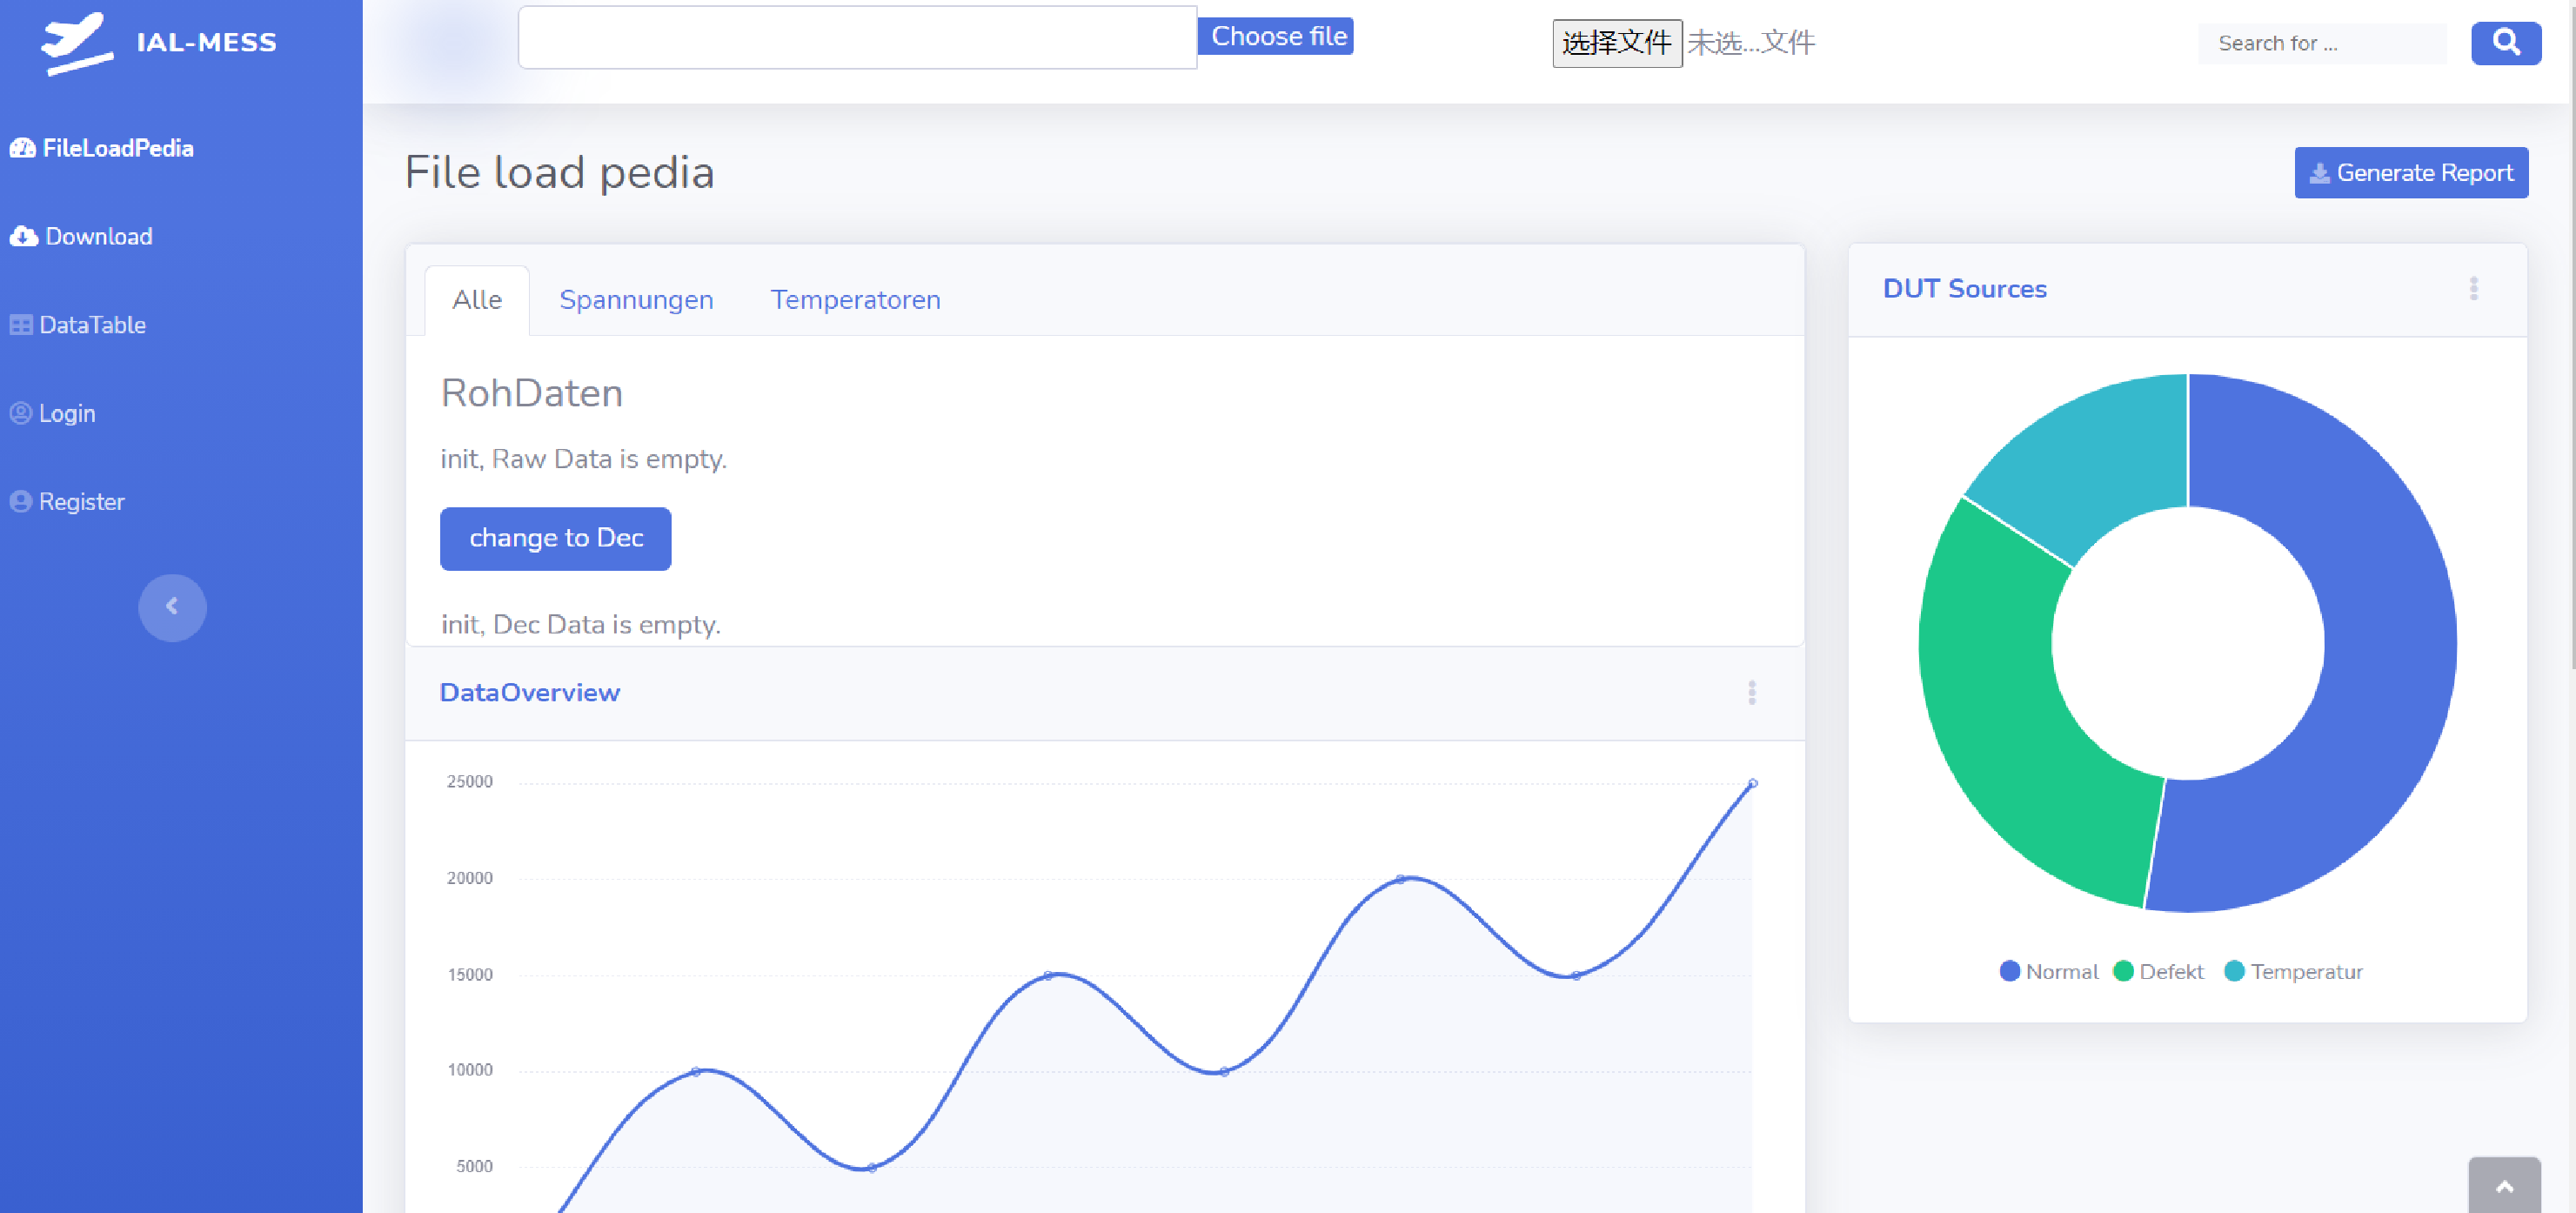
\includegraphics[width=16cm]{grafiken/5.9.pdf}
	\caption{Front end} 
	\label{fig:5.9}
\end{figure}
\FloatBarrier
\\
\chapter{Design PCBs}
\label{chap:Design PCBs}
% 6
The board design of the master and slave is mainly divided into schematic design and package design.

\section{Schematic part from Masterboard and Slaveboard}
\label{sec:Schematic part from Masterboard and Slaveboard}
% 6.1
The main components of the masterboard schematic diagram are the network chip W5500, the microcontroller STM32F429ZG and the corresponding modules, as shown in the following Figure~\ref{fig:6.1}:

\begin{figure}[!ht]
	\centering
	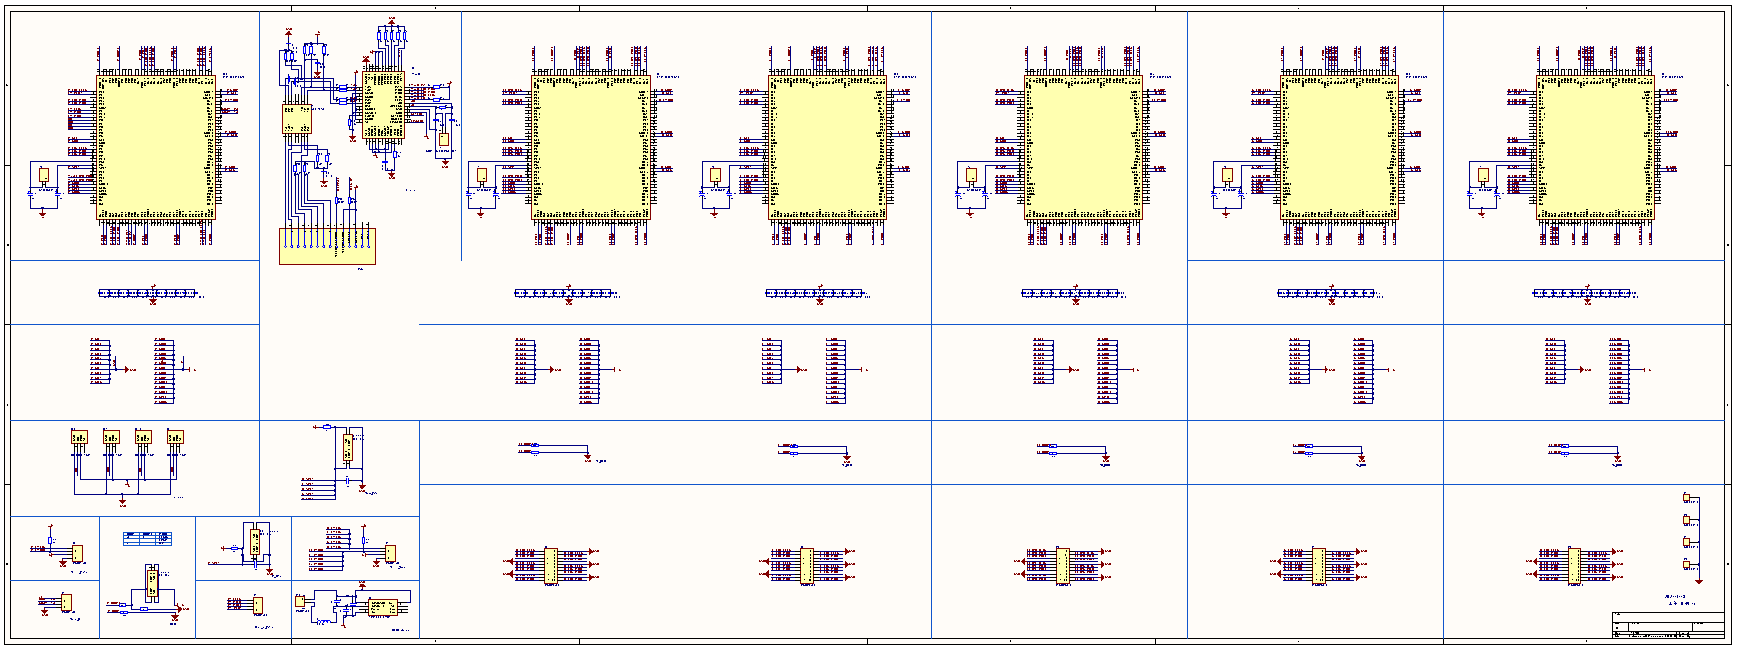
\includegraphics[width=16cm]{grafiken/6.1.pdf}
	\caption{Masterboard schematic diagram} 
	\label{fig:6.1}
\end{figure}
\FloatBarrier
\\

The main components of the slaveboard schematic diagram are the microcontroller STM32F303ZET and the corresponding modules, as shown in the following Figure~\ref{fig:6.2}:

\begin{figure}[!ht]
	\centering
	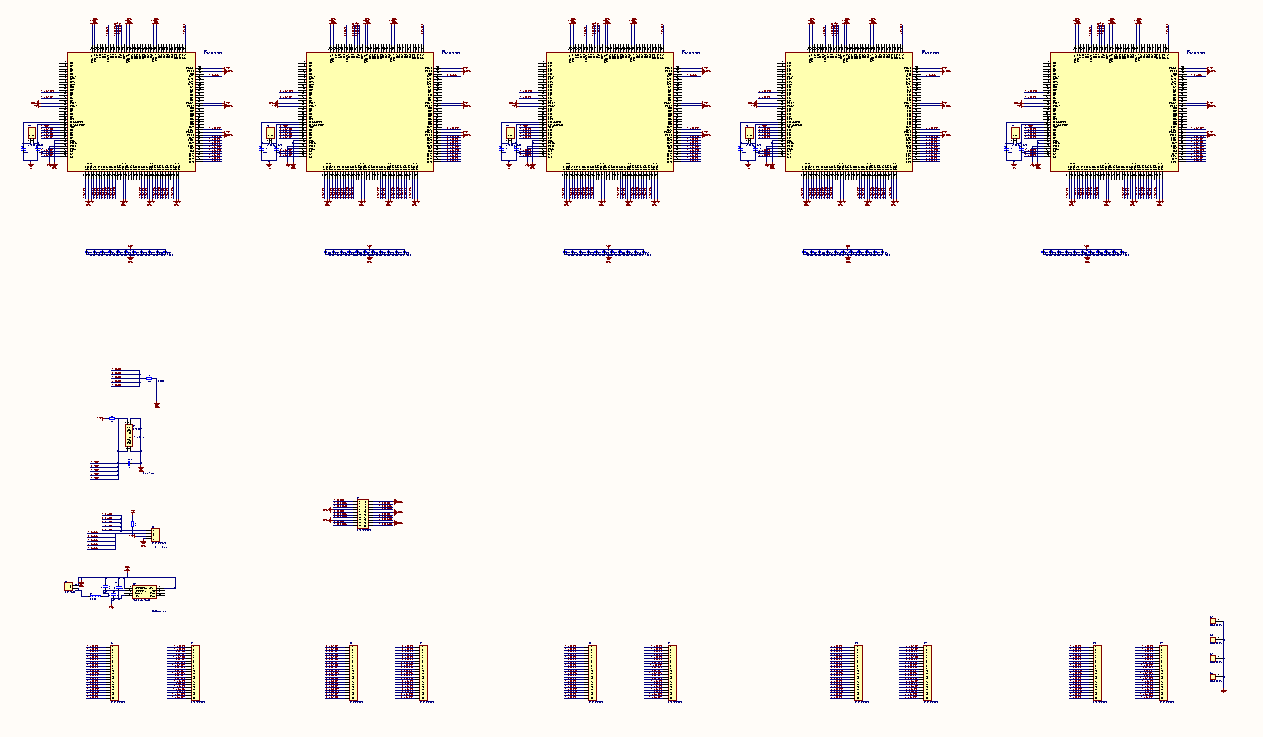
\includegraphics[width=16cm]{grafiken/6.2.pdf}
	\caption{Slaveboard schematic diagram} 
	\label{fig:6.2}
\end{figure}
\FloatBarrier
\\

The Figure~\ref{fig:6.3} below is a schematic diagram of the microcontroller on the masterboard as  Ethernetconnector and a receiver of SPI.

\begin{figure}[!ht]
	\centering
	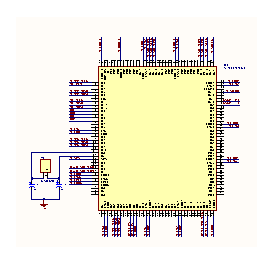
\includegraphics[width=16cm]{grafiken/f429.eps}
	\caption{Stm32F429ZG for Ethernet and Receiver} 
	\label{fig:6.3}
\end{figure}
\FloatBarrier
\\
Corresponding to this, the following Figure~\ref{fig:6.4} is a schematic diagram of the microcontroller on the masterboard as the slave SPI receiver and the Ethernet microcontroller SPI sender.

\begin{figure}[!ht]
	\centering
	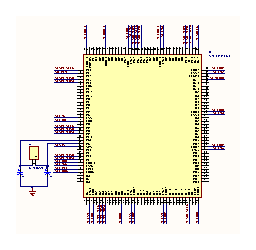
\includegraphics[width=16cm]{grafiken/f429conn.eps}
	\caption{Stm32F429ZG for SPI Receiver/Sender} 
	\label{fig:6.4}
\end{figure}
\FloatBarrier
\\
It is also important that the schematic diagram of the slaveboard mircocontroller is as follows Figure~\ref{fig:6.5}:

\begin{figure}[!ht]
	\centering
	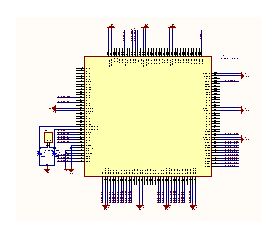
\includegraphics[width=16cm]{grafiken/f303.eps}
	\caption{Stm32F303ZET for SPI Sender and ADC} 
	\label{fig:6.5}
\end{figure}
\FloatBarrier
\\

Each board has a boot circuit, the Figure~\ref{fig:6.6} is as shown below:
\begin{figure}[!ht]
	\centering
	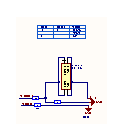
\includegraphics[width=16cm]{grafiken/boot_master.eps}
	\caption{Boot circuit} 
	\label{fig:6.6}
\end{figure}
\FloatBarrier
\\

Each board has a DCDC-Convertor modul, the Figure~\ref{fig:6.7} is as shown below:
\begin{figure}[!ht]
	\centering
	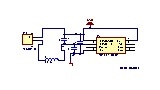
\includegraphics[width=16cm]{grafiken/dcdc.eps}
	\caption{DCDC-Convertor} 
	\label{fig:6.7}
\end{figure}
\FloatBarrier
\\

For UDP communication and signal quality, a network transformer needs to be added when designing the Ethernet module. The Figure~\ref{fig:6.8} of schematic diagram is as follows:
 
\begin{figure}[!ht]
	\centering
	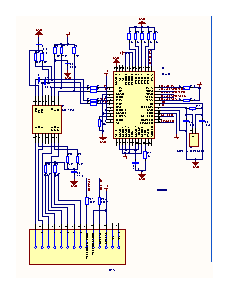
\includegraphics[width=16cm]{grafiken/w5500.eps}
	\caption{Ethernet modul: W5500} 
	\label{fig:6.8}
\end{figure}
\FloatBarrier
\\
While the slave is collecting the voltage signal, the host must collect the temperature signal. The schematic diagram of the temperature sensor DS18b20 is shown in the Figure~\ref{fig:6.9}:

\begin{figure}[!ht]
	\centering
	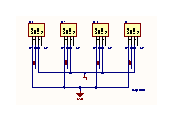
\includegraphics[width=16cm]{grafiken/ds18b20.eps}
	\caption{DS18b20} 
	\label{fig:6.9}
\end{figure}
\FloatBarrier
\\



\section{PCB document design}
\label{sec:PCB document design}
% 6.2
Through the schematic diagram, the package of the schematic diagram can be set and the PCB document can be generated.


\subsection{Layer Stack design}
\label{sec:Layer Stack design}
% 6.2.1

This article produces multi-layer PCB board to ensure signal quality and electromagnetic compatibility. Generally speaking, three kinds of multi-layer board layout modes are illustrated below Figure~\ref{fig:6.10}:
\begin{figure}[!ht]
	\centering
	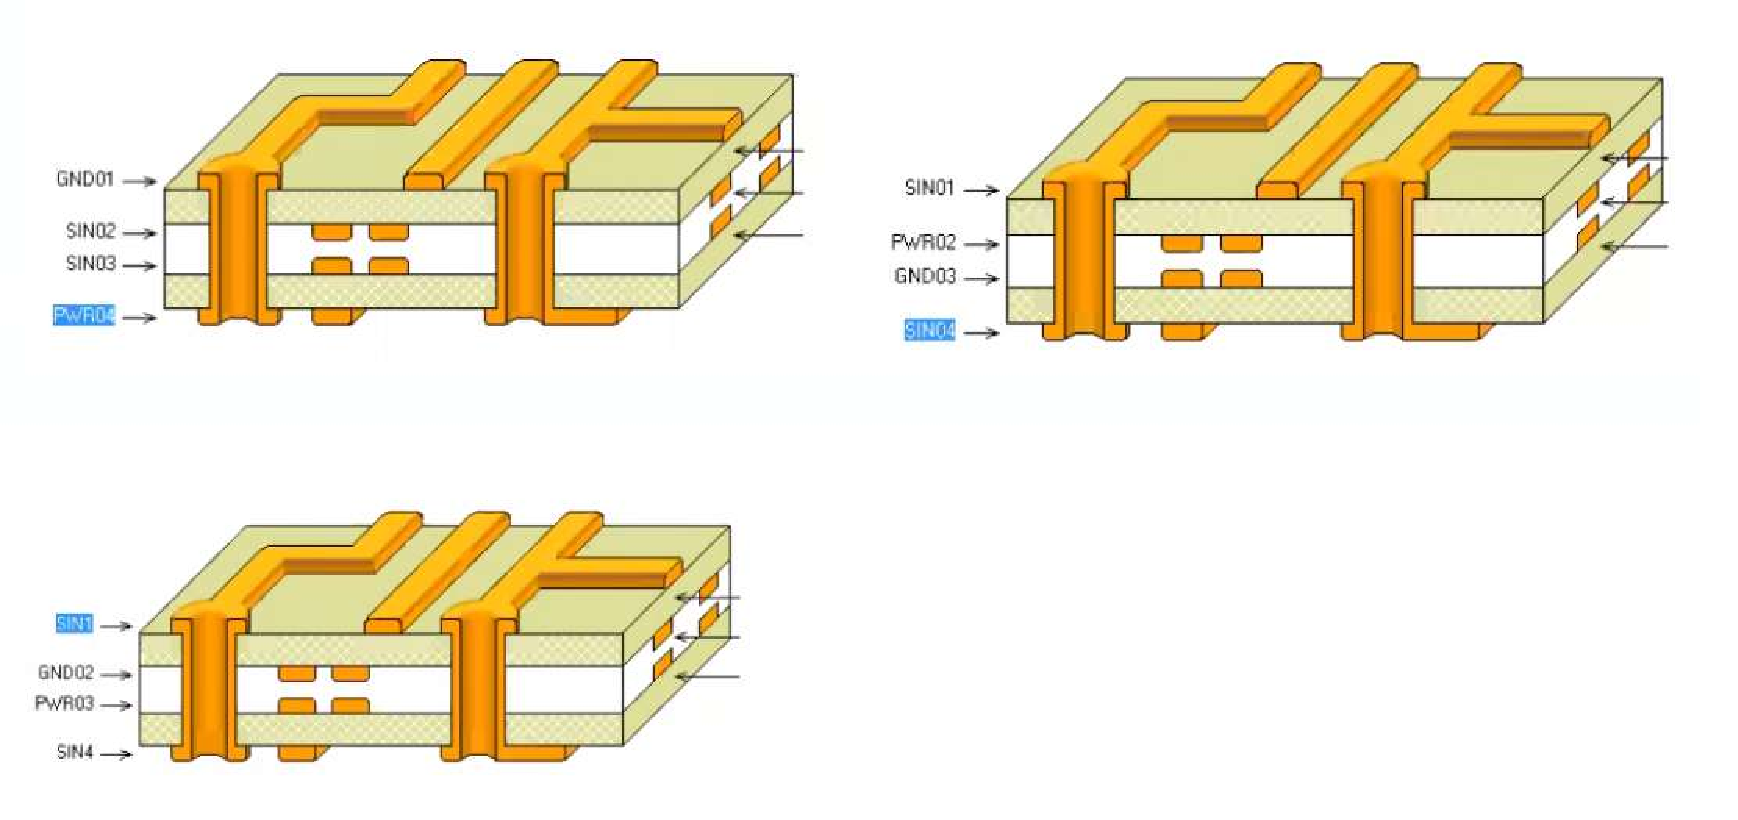
\includegraphics[width=16cm]{grafiken/6.10.pdf}
	\caption{Three common layering methods} 
	\label{fig:6.10}
\end{figure}
\FloatBarrier
\\


Designers need to consider the following four rules according to their needs:
Rule 1: The welding area of the component surface is a complete base plate (Plan A / B / C are OK)
Rule 2: No neighboring parallel wiring layers as far as possible (Plan A is not OK)
Rule 3: All signal layers are as close as possible to the ground plane (Plan B = Plan C)
Rule 4: The key signal is next to the floor and does not cross the partition (Plan B is not OK)
In our measurement, Plan C is best. It’s also because the amount of signals we transmit is large and it takes a long time to use.
The Figure~\ref{fig:6.11} below is the third plan to expand the Layer Stack method of eight-layer PCB:

% fig6.11
\begin{figure}[!ht]
	\centering
	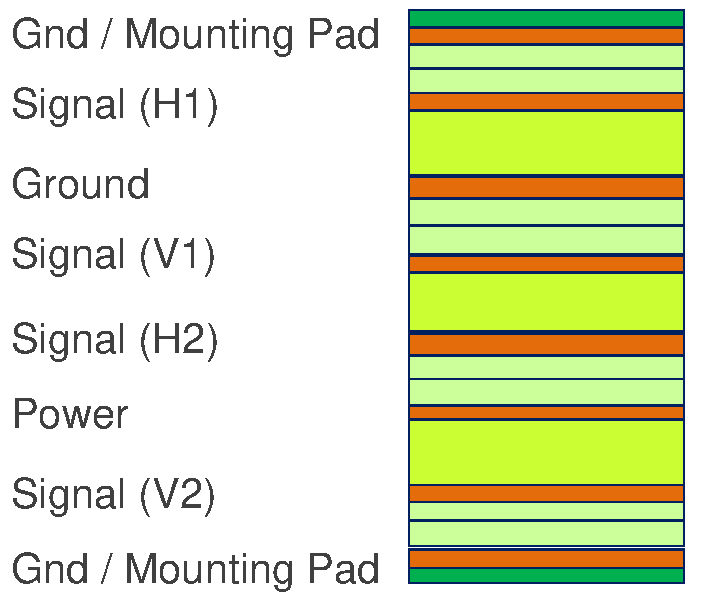
\includegraphics[width=16cm]{grafiken/6.11.pdf}
	\caption{Selected layering method} 
	\label{fig:6.11}
\end{figure}
\FloatBarrier
\\

\subsection{PCB Rules}
\label{sec:PCB Rules}
% 6.2.1
The designer needs to consider two rules below. 
Rule1: 20H
When the pcb board has many layers, the power layer and the ground layer will generate electromagnetic waves as shown in the figure below, we can reduce the area of the power layer to reduce the radiated electromagnetic waves.
Edge effect: RF (Radio Freq) wave interference
100H: Reduce 98$\%$ of the external radiation and interference on yourself
20H: Reduce 90$\%$ of the external radiation and interference on yourself
The following Figure~\ref{fig:6.13} is the 20H rule:
~\ref{fig:6.12}
% fig6.12
\begin{figure}[!ht]
	\centering
	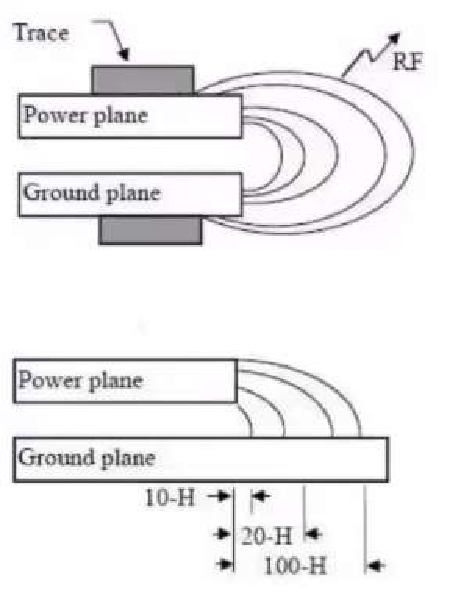
\includegraphics[width=16cm]{grafiken/6.12.pdf}
	\caption{Rule:20H} 
	\label{fig:6.12}
\end{figure}
\FloatBarrier
\\

Rule2: 3M
If the distance between the two signal lines is too small, crosstalk will occur, and it is difficult to ensure a high signal-to-noise ratio, so this article introduces design rules: 3M (3mil)
% fig6.13
The following Figure~\ref{fig:6.13} is the 3M rule:

\begin{figure}[!ht]
	\centering
	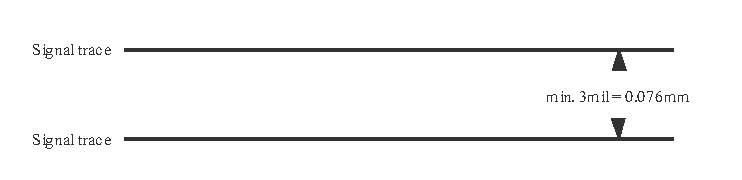
\includegraphics[width=16cm]{grafiken/6.13.pdf}
	\caption{Rule:3M} 
	\label{fig:6.13}
\end{figure}
\FloatBarrier
\\


The following pictures are the PCB document of the masterboard Figure~\ref{fig:6.14} Figuren~\ref{fig:6.15} and the PCB document of the slaveboard Figure~\ref{fig:6.16} Figure~\ref{fig:6.17}.

\begin{figure}[!ht]
	\centering
	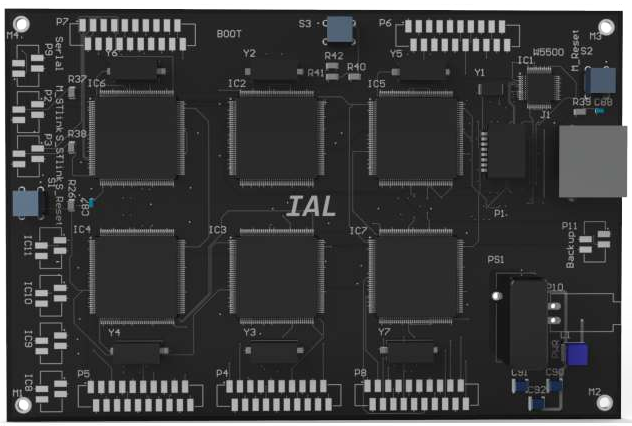
\includegraphics[width=16cm]{grafiken/6.14.pdf}
	\caption{Masterboard PCB document front view} 
	\label{fig:6.13}
\end{figure}
\FloatBarrier
\\


\begin{figure}[!ht]
	\centering
	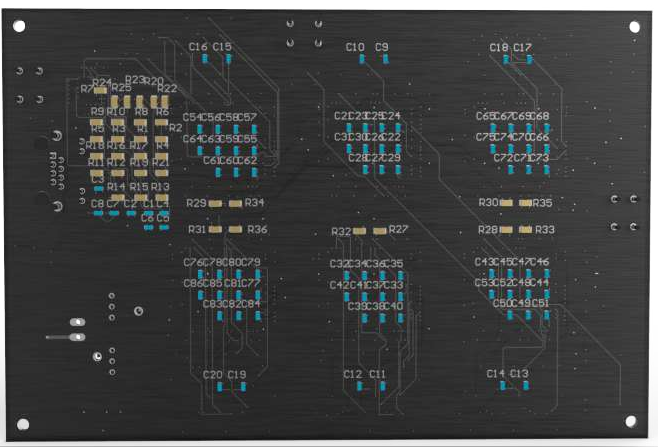
\includegraphics[width=16cm]{grafiken/6.15.pdf}
	\caption{Masterboard PCB document back view} 
	\label{fig:6.15}
\end{figure}
\FloatBarrier
\\


\begin{figure}[!ht]
	\centering
	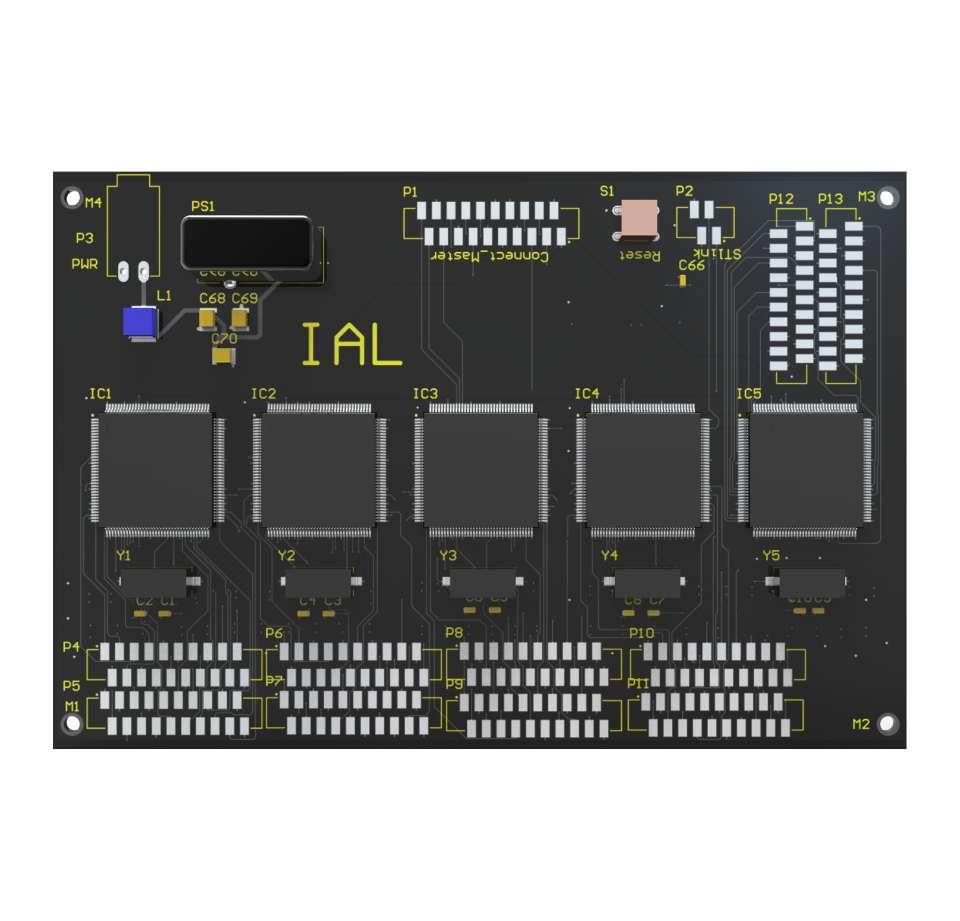
\includegraphics[width=16cm]{grafiken/6.16.pdf}
	\caption{Slaveboard PCB document front view} 
	\label{fig:6.16}
\end{figure}
\FloatBarrier
\\


\begin{figure}[!ht]
	\centering
	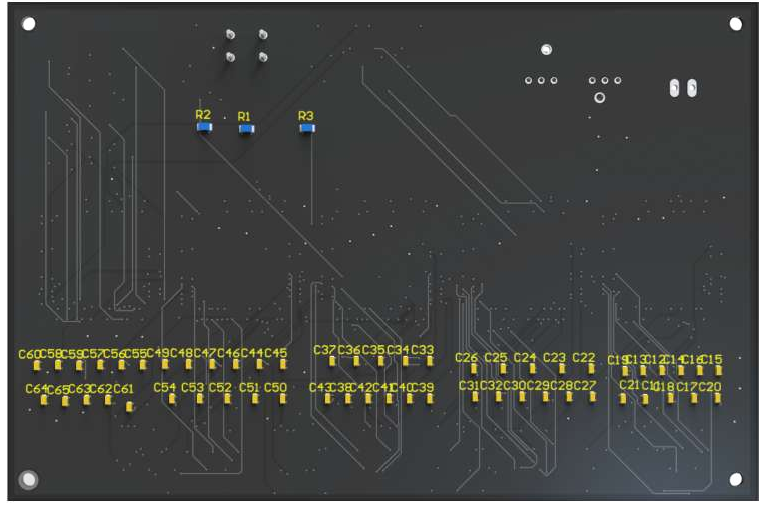
\includegraphics[width=16cm]{grafiken/6.17.pdf}
	\caption{Slaveboard PCB document back view} 
	\label{fig:6.17}
\end{figure}
\FloatBarrier
\\



\chapter{Introduce measurement with eval boards }
\label{chap:Introduce measurement with eval boards }
% 7
 

\chapter{Conlusion}
\label{chap:Conlusion}
% 8.x
In order to measure the effects of cosmic radiation on GaN power semiconductors for a long time, the microcontroller STM32F303 is used to measure the voltage signal and the DS18b20 is used to measure the temperature signal.
\\
The collected signal is sent to the main control unit of the microprocessor through AD conversion, the data collection stage is realized through database and back-end processing, and the collected data is sent to the front-end to facilitate clearly understanding of the users.
The acquisition circuit is also simulated at the same time, the PCB board is designed and laid out to meet the design requirements.
\\
Researchers can first debug the data which is collected from the host and slave through the debugger, then import the collected data into the MySQL database through the shell command line, and finally convert the IP address of the intranet to the public network address through the intranet penetration. In this case the personnel at the Hannover Institute can also observe changes of the collected signals such as the number of failed units under test. Researchers can also remotely access and control the experimental PC through VNC and collect data from the back-end to the database and then to the front-end. This realized the process of the Internet of Things.



% \subsection{Simulation of Measurement circuit}
% \label{sec:Simulation of Measurement circuit}
% % 3.x.x

% \section{ }
% \label{sec: }
% % 3.x
  
% \section{Calculation of acquisition speed}
% \label{sec:Calculation of acquisition speed}
% % 4.4
% To improve reliability and SNR, this article needs to discuss the upper limit of acquisition speed to ensure that all data will be sent to the PC correctly. 
% \\
% According to the chip’s specification, SPI of the slave only has the fastest transmission speed of 4Mbps. Moreover, four slave mainboards send data to the host mainboard. Every time, ADC voltage signal acquisition at least needs 1.5 periods and the maximum periods should be set up as 601.5. According to the specification, each switching time is: 



 


